% BU ECE template for MS thesis and PhD dissertation.
%
%==========================================================================%
% MAIN PREAMBLE 
%==========================================================================%
\documentclass[12pt,letterpaper]{report}          % Single-sided printing for the library
%\documentclass[12pt,twoside]{report} % Double-sided printing
\usepackage[intlimits]{amsmath}
\usepackage{amsfonts,amssymb,amsthm}
\DeclareSymbolFontAlphabet{\mathbb}{AMSb}
%\usepackage{natbib}
\usepackage{apalike}
\usepackage{float}
\usepackage[bf]{caption}       
\setcaptionmargin{0.5in}
\usepackage{fancyhdr}
%\usepackage{fancyheadings}
\usepackage{fancybox}
\usepackage{ifthen}
\usepackage{bu_ece_thesis}
\usepackage{url}
\usepackage{lscape,afterpage}
\usepackage{xspace}
\usepackage{epstopdf} 
\usepackage{subfig}

%==========================================================================%
%%% graphicx and pdf creation
\usepackage{graphicx}
\usepackage{appendix}
%\usepackage{psfrag}
%\DeclareGraphicsExtensions{.eps}   % extension for included graphics
%\usepackage{thumbpdf}              % thumbnails for ps2pdf
%\usepackage[ps2pdf,                % hyper-references for ps2pdf
%bookmarks=true,%                   % generate bookmarks ...
%bookmarksnumbered=true,%           % ... with numbers
%hypertexnames=false,%              % needed for correct links to figures !!!
%breaklinks=true,%                  % breaks lines, but links are very small
%linkbordercolor={0 0 1},%          % blue frames around links
%pdfborder={0 0 112.0}]{hyperref}%  % border-width of frames 
%                                   % will be multiplied with 0.009 by ps2pdf
%\hypersetup{
%  pdfauthor   = {Joe Graduate <joe.graduate@bu.edu>},
%  pdftitle    = {dissertation.pdf},
%  pdfsubject  = {doctoral dissertations},
%  pdfkeywords = {mathematics, science, technology},
%  pdfcreator  = {LaTeX with hyperref package},
%  pdfproducer = {dvips + ps2pdf}
%}
\usepackage{cleveref}
%==========================================================================%
% customized commands can be placed here
\newcommand{\mcX}{\mathcal{X}}
\newcommand{\mcU}{\mathcal{U}}
\newcommand{\mcQ}{\mathcal{Q}}

% Common sets
\newcommand{\Z}{\mathbb{Z}}
\newcommand{\R}{\mathbb{R}}
\newcommand{\N}{\mathbb{N}}

% Environements
\newtheorem{defn}{Definition}
\newtheorem{prop}{Proposition}
\newtheorem{lem}{Lemma}
\newtheorem{theorem}{Theorem}
\newtheorem{assum}{Assumption}

\crefname{lem}{lemma}{lemmas}
\Crefname{lem}{Lemma}{Lemmas}
\crefname{assum}{assumption}{assumptions}
\Crefname{assum}{Assumption}{Assumptions}
%==========================================================================%

%==========================================================================%
% BEGIN
%==========================================================================%
\begin{document}
	
	% The preliminary pages
	% !TeX root = ../thesis.tex
% This file contains all the necessary setup and commands to create
% the preliminary pages according to the buthesis.sty option.

\title{Kink-like Solutions for the FPUT Lattice and the mKdV as a Modulation Equation}
\author{Trevor Norton}

% Type of document prepared for this degree:
%   1 = Master of Science thesis,
%   2 = Doctor of Philisophy dissertation.
%   3 = Master of Science thesis and Doctor of Philisophy dissertation.
\degree=2

\prevdegrees{B.S., Virginia Polytechnic Institute and State University, 2015\\
	M.S., Virginia Polytechnic Institute and State University, 2018}

\department{Department of Mathematics and Statistics}

% Degree year is the year the diploma is expected, and defense year is
% the year the dissertation is written up and defended. Often, these
% will be the same, except for January graduation, when your defense
% will be in the fall of year X, and your graduation will be in
% January of year X+1
\defenseyear{2023}
\degreeyear{2023}

% For each reader, specify appropriate label {First, Second, Third},
% then name, and title. IMPORTANT: The title should be:
%   "Professor of Electrical and Computer Engineering",
% or similar, but it MUST NOT be:
%   Professor, Department of Electrical and Computer Engineering"
% or you will be asked to reprint and get new signatures.
% Warning: If you have more than five readers you are out of luck,
% because it will overflow to a new page. You may try to put part of
% the title in with the name.
\reader{First}{C. Eugene Wayne, PhD}{Professor of Mathematics}
\reader{Second}{Tasso Kaper, PhD}{Professor of Mathematics}
\reader{Third}{Margaret Beck, PhD}{Professor of Mathematics}
\reader{Fourth}{Ryan Goh, PhD}{Assistant Professor of Mathematics}

% The Major Professor is the same as the first reader, but must be
% specified again for the abstract page. Up to 4 Major Professors
% (advisors) can be defined. 
\numadvisors=1
\majorprof{C. Eugene Wayne, PhD}{{Professor of Mathematics}}
%\majorprofb{First M. Last, PhD}{{Professor of Astronomy}}
%\majorprofc{First M. Last, PhD}{{Professor of Biomedical Engineering}}

%%%%%%%%%%%%%%%%%%%%%%%%%%%%%%%%%%%%%%%%%%%%%%%%%%%%%%%%%%%%%%%%  

%                       PRELIMINARY PAGES
% According to the BU guide the preliminary pages consist of:
% title, copyright (optional), approval,  acknowledgments (opt.),
% abstract, preface (opt.), Table of contents, List of tables (if
% any), List of illustrations (if any). The \tableofcontents,
% \listoffigures, and \listoftables commands can be used in the
% appropriate places. For other things like preface, do it manually
% with something like \newpage\section*{Preface}.

% This is an additional page to print a boxed-in title, author name and
% degree statement so that they are visible through the opening in BU
% covers used for reports. This makes a nicely bound copy. Uncomment only
% if you are printing a hardcopy for such covers. Leave commented out
% when producing PDF for library submission.
%\buecethesistitleboxpage

% Make the titlepage based on the above information.  If you need
% something special and can't use the standard form, you can specify
% the exact text of the titlepage yourself.  Put it in a titlepage
% environment and leave blank lines where you want vertical space.
% The spaces will be adjusted to fill the entire page.
\maketitle
\cleardoublepage

% The copyright page is blank except for the notice at the bottom. You
% must provide your name in capitals.
\copyrightpage
\cleardoublepage

% Now include the approval page based on the readers information
\approvalpage
\cleardoublepage

% Here goes your favorite quote. This page is optional.
%\newpage
%\thispagestyle{empty}
%\phantom{.}
\vspace{4in}

\begin{singlespace}
\begin{quote}
  \textit{Facilis descensus Averni;}\\
  \textit{Noctes atque dies patet atri janua Ditis;}\\*
  \textit{Sed revocare gradum, superasque evadere ad auras,}\\
  \textit{Hoc opus, hic labor est.}\hfill{Virgil (from Don's thesis!)}
\end{quote}
\end{singlespace}

% \vspace{0.7in}
%
% \noindent
% [The descent to Avernus is easy; the gate of Pluto stands open night
% and day; but to retrace one's steps and return to the upper air, that
% is the toil, that the difficulty.]

%\cleardoublepage

% The acknowledgment page should go here. Use something like
% \newpage\section*{Acknowledgments} followed by your text.
\newpage
\section*{\centerline{Acknowledgments}}
% !TeX root = ../thesis.tex

I would like to thank my advisor, Gene, for all his help with this thesis. He originally suggested the topic of research, and since then he has been giving guidance and feedback on my work. This thesis would not have been possible without his help, and I greatly appreciated having him as an advisor.

%Thank the committee 

%Thank Julio and Mark

%Thank my parents

%Thank Stuart

This research was supported in part by the US National Science Foundation through grant DMS-1813384 whose assistance is gratefully acknowledged.


%\vskip 1in

%\noindent
%Janusz Konrad\\
%Professor\\
%ECE Department
\cleardoublepage

% The abstractpage environment sets up everything on the page except
% the text itself.  The title and other header material are put at the
% top of the page, and the supervisors are listed at the bottom.  A
% new page is begun both before and after.  Of course, an abstract may
% be more than one page itself.  If you need more control over the
% format of the page, you can use the abstract environment, which puts
% the word "Abstract" at the beginning and single spaces its text.

\begin{abstractpage}
% !TeX root = ../thesis.tex
% ABSTRACT

[This is where the text for the abstract will go]

\end{abstractpage}
\cleardoublepage

% Now you can include a preface. Again, use something like
% \newpage\section*{Preface} followed by your text

% Table of contents comes after preface
\tableofcontents
\cleardoublepage

% If you do not have tables, comment out the following lines
%\newpage
%\listoftables
%\cleardoublepage

% If you have figures, uncomment the following line
%\newpage
%\listoffigures
%\cleardoublepage

% List of Abbrevs is NOT optional (Martha Wellman likes all abbrevs listed)
\chapter*{List of Abbreviations}
\begin{center}
  \begin{tabular}{lll}
    \hspace*{2em} & \hspace*{1in} & \hspace*{4.5in} \\
    FPUT  & \dotfill & Fermi-Pasta-Ulam-Tsingou \\
    KdV & \dotfill & Korteweg-de Vries \\
    mKdV  & \dotfill & modified Korteweg-de Vries\\
  \end{tabular}
\end{center}
\cleardoublepage

% END OF THE PRELIMINARY PAGES

\newpage
\endofprelim
        
	\cleardoublepage
	
	% -------------------------------------
	% CHAPTER ?: LONG-TIME STABILITY OF SMALL FPU SOLITARY WAVES
	% -------------------------------------
	% !TeX root = ../thesis.tex
\chapter{Long-Time approximations of small-amplitude, long-wavelength  FPUT solutions}
\label{chp:long-time-stability}
\pagestyle{myheadings}

\section{Introduction}

As shown in earlier work, there exists a wave solution of the FPUT lattice whose profile is well approximated by that of the kink solution to the (defocusing) mKdV. This approximation holds globally in time, but is restricted to one special solution of the FPUT. We are now interested in studying more general solutions of the FPUT which can be approximated by solutions of the mKdV for long (but finite) time. The equations of motion on the lattice are given by 
\begin{equation*}
	\ddot x_n = V'(x_{n+1} - x_n) - V'(x_n - x_{n-1}), \quad n \in \Z. \tag{\ref{fput-lattice-odes}}
\end{equation*}
where \(V\) is the interaction potential between neighboring particles and \(\dot{\hspace{0.5em}}\) denotes the derivative with respect to the time \(t\in \mathbb{R}\). \Cref{fput-lattice-odes} can be rewritten in the strain variables \(u_n := x_{n+1} - x_n\) as follows
\begin{equation*}
	\ddot{u}_n = V'(u_{n+1}) - 2 V'(u_n) + V'(u_{n-1}), \quad n \in \Z \tag{\ref{fput-lattice-equations-strain-variables}}
\end{equation*}
The moving wave solution in \cref{fput-lattice-odes} corresponds to a kink-like solution in \cref{fput-lattice-equations-strain-variables}.

For the case where \(V\) is of the form \(V(u) = \frac 1 2 u^2 + \frac{\epsilon^2}{p+1} u^{p+1}\) for \(p\geq 2\), the generalized KdV equation given by 
\begin{equation}\label{generalized-KdV}
	2 \partial_TW + \frac 1 {12} \partial_X^3 W + \partial_X(W^p) = 0,\quad X\in\R
\end{equation} 
serves as a modulation equation for solutions of \cref{fput-lattice-equations-strain-variables} \cite{bambusi2006metastability,friesecke1999solitary}. That is, for a local solution \(W\in C([-\tau_0,\tau_0],H^s(\R))\) of \cref{generalized-KdV} there exist positive constants \(\epsilon_0\) and \(C_0\) such that, for all \(\epsilon \in (0,\epsilon_0)\), when initial data \((u_{\mathrm{in} }, \dot u_{\mathrm{in}})\in\ell^2(\R)\) satisfy
\begin{equation}
	\|u_{\mathrm{in}} - W(\epsilon\cdot, 0) \|_{\ell^2} + \| \dot u_{\mathrm{in}} + \epsilon \partial_X W(\epsilon\cdot, 0) \|_{\ell^2} \leq \epsilon^{3/2},
\end{equation}
the unique solution to \cref{fput-lattice-equations-strain-variables} with initial data \((u_{\mathrm{in} }, \dot u_{\mathrm{in}})\) belongs to \(C^1([-\tau_0\epsilon^{-3}, \tau_0 \epsilon^{-3}];\allowbreak \ell^2(\Z))\) and satisfies 
\begin{multline}
	\|u(t) - W(\epsilon (\cdot - t),\epsilon^3 t)\|_{\ell^2(\Z)} + \| \dot u(t) + \epsilon \partial_X W(\epsilon(\cdot - t), \epsilon^3 t) \|_{\ell^2(\Z)} \leq C_0 \epsilon^{3/2}, \\ t\in[-\tau_0 \epsilon^{-3},\tau_0 \epsilon^{-3}].
\end{multline}
Furthermore, the approximation can also be extended to include counter-propagating solutions of the KdV in the case where \(p=2\) \cite{schneider2000counter,hong2021korteweg}.

The KdV approximation was extended to longer time scales on the order of \(\epsilon^{-3}|\log(\epsilon)|\) by Khan and Pelinovsky in order to deduce the nonlinear metastability of small FPUT solitary waves from the orbital stability of the corresponding KdV solitary waves \cite{khan2017long}.

We consider the FPUT with potential
\begin{equation}\label{truncated-potential}
	V(u) = \frac 1 2 u^2 - \frac{1} {24} u^4.
\end{equation}
This potential differs from those studied in \cite{khan2017long} in that it admits kink solutions. Numerical experiments show that these kink solutions play an important role in the FPUT recurrence for lattices with potential give in \cref{truncated-potential} \cite{pace2019beta}. We will introduce an ansatz that solutions of the FPUT with this potential can be well-approximated by counter-propagating solutions of mKdV equations.

The technique of the proof follows from ideas in \cite{schneider2000counter,khan2017long} and is roughly sketched out as follows. First the system is rewritten into a Hamiltonian system on a Hilbert space, \(H\):
\begin{equation}\label{hamiltonian-system}
	\dot X(t) = J \mcH'(X)
\end{equation}
where \(J:H\to H\) is a skew symmetric operator and \(\mcH\) is the Hamiltonian such that \(\mcH'(X) = LX + N(X)\) with \(L:= \mcH'(0)\). We introduce some ansatz \(\tilde X_\epsilon\) which is an approximate solution to \cref{hamiltonian-system} in the sense that 
\begin{equation}
	\mathrm{Res}(t) := J[L\tilde X_\epsilon(t)  + N(\tilde X_\epsilon(t))] - \dot{\tilde {X_\epsilon}}(t) 
\end{equation}
has norm of order \(\epsilon^\alpha\) for \(\alpha > 0\)  for all time \(t\). The approximate solution will be ``small-amplitude" in the sense that \(\| \tilde X_\epsilon \| = \mathcal O(\epsilon^k)\) for \(k > 0 \). Then we can write the evolution equation for the \(R(t) = X(t) - \tilde X_\epsilon(t)\) as 
\begin{equation}\label{hamiltonian-system-2}
	\dot R(t) = J[L + N'(\tilde X_\epsilon(t))]R(t) + \mathrm{Res}(t) + \mathcal N(\tilde X_\epsilon, R)
\end{equation}
with \(\mathcal N( X_\epsilon, R) := J[N(\tilde X_\epsilon +R) - N(\tilde X_\epsilon) - N'(\tilde X_\epsilon)R]\). The goal is then to show that \(R(t)\) remains small for long periods of time so that the approximation \(X \approx \tilde X_\epsilon\) is valid for that time. The standard way to prove this is to find a suitable energy function to control the norm of \(R\) with. If \(L + N'(\tilde X_\epsilon(t))\) is self-adjoint, then \cref{hamiltonian-system-2} is up to first order a linear, non-autonomous, Hamiltonian system with Hamiltonian \(\mcH_1(R, t) = \frac 1 2 \langle (L+N'(\tilde X_\epsilon)) R, R\rangle\). Therefore, \(\mcE(t) := \mcH_1(R(t),t)\) serves as a natural choice of energy function for \cref{hamiltonian-system-2}. Hence, if one shows that \( \| R\|^2\lesssim\mcE(t)\) and that  \(\|\mathcal N(\tilde X_\epsilon, R) \| \lesssim \epsilon^{k+2} \mcE(t)\), then can show that \(\mcS(t) = \mcE(t)^{1/2}\) satisfies
\begin{equation}
	|\dot \mcS (t) | \lesssim \epsilon^{\alpha} + \epsilon^{k+2}\mcS(t).
\end{equation}
Intuitively, one would expect \(\mcS(t)\) to grow like \(\mcS(t) \sim \epsilon^\alpha t + e^{\epsilon^{k+2} t} \mcS(0)\). Taking \(\mcS(0) =\epsilon^\gamma\) for \(\gamma \geq 1\) and assuming \(\alpha > 2(k+2)\), we have \(\mcS(t) \sim \epsilon^\gamma \) for \(|t|\lesssim \epsilon^{-(k+2)}\). One can further the time where the approximation holds by relaxing how big \(\mcS(t)\) can get. Taking \(r>0\) small, one can show that \(\mcS(t) \sim \epsilon^{\gamma - r}\) for \(|t| \lesssim r \epsilon^{-(k+2)}|\log(\epsilon)|\).

%Something about metastability here.

\section{Counter-Propagating Waves Ansatz}

%Write out counter-propagting ansatz for solution 
We make the assumption that solutions of \cref{fput-lattice-equations-strain-variables} can be expressed as a sum of two counter-propagating small-amplitude waves, i.e., 
\begin{equation}\label{ansatz}
	u_n(t) \approx \epsilon f(\epsilon(n+t), \epsilon^3t) + \epsilon g(\epsilon(n-ct), \epsilon^3 t) + \epsilon^3\phi(\epsilon n, \epsilon t)
\end{equation}
where we allow \(f\) to have a fixed non-zero limits, \(f_{\pm\infty}\), at positive and negative infinity and \(\phi\) captures the interaction effects between \(f\) and \(g\). The wave speed of \(g\) is given by
\begin{equation}\label{ansatz-wave-speed}
	c = c(\epsilon, f_\infty) = 1 - \frac{\epsilon^2 f_\infty^2}{4}.
\end{equation}
Plugging in the ansatz in \cref{ansatz} back into \cref{fput-lattice-equations-strain-variables} and grouping terms of the same order \(\epsilon\) together gives
\begin{equation}
	\begin{aligned}
		&\epsilon^3 \Big(\partial_1^2 f(\cdot, \epsilon^3 t) + \partial_1^2 g(\cdot, \epsilon^3 t)\Big) \\
		&+ \epsilon^5 \Big( 2 \partial_1\partial_2 f(\cdot, \epsilon^3t) - 2 \partial_1\partial_2 g(\cdot, \epsilon^3 t) - \frac{f_\infty^2} 2 \partial_1^2 g + \partial_2^2 \phi(\epsilon x, \epsilon t)\Big) \\
		&+ \mathcal O(\epsilon^6)\\
		&\qquad = \quad \epsilon^3 \Big(\partial_1^2 f(\cdot, \epsilon^3 t) + \partial_1^2 g(\cdot, \epsilon^3 t)\Big) \\
		&\qquad\qquad + \epsilon^5\Big(\partial_1^2  \phi(\epsilon x, \epsilon t) \\
		&\qquad\qquad\qquad - \frac 1 6 \partial_1^2 \big[f^3(\cdot, \epsilon^3 t ) + 3 f^2(\cdot,\epsilon^3)g(\cdot, \epsilon^3t) + 3 f(\cdot, \epsilon t) g^2(\cdot,\epsilon^3 t) + g^3(\cdot, \epsilon^3 t)\big] \\
		&\qquad\qquad\qquad+ \frac 1 {12} \partial_1^4 f(\cdot, \epsilon^3 t) + \frac 1 {12} \partial_1^4 g(\cdot, \epsilon^3 t)\Big) \\
		&\qquad\qquad+ \mathcal O(\epsilon^6).
	\end{aligned}
\end{equation}
Clearly the equation will hold up to order \(\epsilon^3\). For the order \(\epsilon^5\) terms, the equation will again hold if \(f\), \(g\), and \(\phi\) satisfy
\begin{equation}\label{f-mKdV}
	2 \partial_2 f = - \frac 1 6 \partial_1(f^3) + \frac 1 {12} \partial_1^3 f
\end{equation}
and 
\begin{equation}\label{g-gKdV}
	-2 \partial_2 g = - \frac 1 6 \partial_1 (g^3 + 3f_\infty g^2) + \frac 1 {12}\partial_1^3 g,
\end{equation}
and
\begin{equation}\label{phi-pde}
	\begin{aligned}
		\partial_2^2 \phi(\xi, \tau) = \partial_1^2\phi(\xi, \tau)- \frac 1 6 \partial_1^2 \big[& 3(f^2(\xi+\tau,\epsilon^2\tau)-f_\infty^2)g(\xi-c\tau,\epsilon^2\tau) \\&+ 3 (f(\xi+\tau,\epsilon^2\tau)-f_\infty)g^2(\xi-c\tau,\epsilon^2\tau) \big ] \\
		\phi(\xi,0) = \partial_1 \phi(\xi, 0) = 0.
	\end{aligned}
\end{equation}
Note that \cref{f-mKdV} is the defocusing mKdV equation and \cref{g-gKdV} is a type of generalized KdV equation. This formal calculation shows that the mKdV can serve as a modulation equation. That is, for \(\epsilon\) sufficiently small, one would expect the ansatz in \cref{ansatz} to hold for time on the order of \(\epsilon^{-3}\). We make precise this notion, but we must first make decisions for the function spaces in which the functions \(f\), \(g\), and \(\phi\) must live.

A natural choice of function space for \(g\) is a Sobolev space like \(H^k(\R)\). However, for \(f\), we want to allow the possibility of the function approaching a non-zero limit at positive and negative infinity while also having sufficient regularity. 
\begin{defn}
	For \(k\in\N\), let \(\mcX^k(\R)\) be the Banach space 
	\begin{equation}
		\mcX^k(\R) := \{f \in L^\infty(\R) \mid f'\in H^{k-1}(\R)\}
	\end{equation}
	with norm
	\begin{equation}
		\| f \|_{\mcX^k(\R)} := \| f \|_{L^\infty(\R)} + \| f' \|_{H^{k-1}(\R)}.
	\end{equation}
\end{defn}
Then \(\mcX^k\) is the set of \(L^\infty\) functions which are \(k\) times weakly differentiable and whose derivatives are in \(L^2\). That this is a Banach space follows from the Banach space isomorphism
\begin{equation}
	\mcX^k(\R) \cong L^\infty(\R) \cap \dot H^1(\R) \cap \dot H^k(\R),
\end{equation}
where \(\dot H^k(\R)\) denotes the homogeneous Sobolev spaces. For convenience, we let \(\mcX^0(\R)\) denote \(L^\infty(\R)\)

Note that \cref{f-mKdV} has kink solutions of the form
\begin{equation}\label{kink-solutions}
	f(X,T) = - \sqrt{12 v} \tanh\left( \sqrt{12v} (X-vT)\right).
\end{equation}
In particular, setting \(v = 24\) we get the approximate solution on the lattice given by
\begin{equation}
	- \frac \epsilon {\sqrt 2} \tanh\left(\frac \epsilon {\sqrt 2} \left(n + \left(1-\frac{\epsilon^2} {24}\right) t\right)\right),
\end{equation} which seems to agree with the kink solution on the lattice for long periods of time (i.e.\ it should hold formally for \(t\) of order \(\mathcal O(\epsilon^{-4})\)). The space \(\mcX^k\) allows for \(f\) to be these kink solutions and thus allows us to study the kink solution of the lattice found previously. 

We also have the following inequalities for products of functions in \(\mcX^k\) and \(H^k\) that will be useful. 

	
\begin{restatable}{lem}{prodruleone}
	\label{prod-rule-1-lem}
	For non-negative integers \(k\), there is a \(C>0\) such that
	\begin{equation}\label{prod_rule}
		\| fg \|_{H^k} \leq C \| f \|_{\mathcal X^k} \| g \|_{H^k}
	\end{equation}
	for any \(f\in \mcX^k(\mathbb R)\) and \(g \in H^k(\mathbb R)\).
\end{restatable}

\begin{restatable}{lem}{prodruletwo}
	\label{prod-rule-2-lem}
	For non-negative integers \(k\), there is a \(C>0\) such that
	\begin{equation}\label{prod_rule_2}
		\| fg \|_{\mcX^k} \leq C \| f \|_{\mcX^k} \| h \|_{\mcX^k}
	\end{equation}
	for any \(f,g\in \mcX^k(\mathbb R)\).
\end{restatable}
See \cref{lemma-appendix} for proofs.

However, for our main result, we require that \(\phi\), the term which captures the interaction effects, remains uniformly bounded for all time. Intuitively, if \(f\) and \(g\) are localized, the inhomogeneous term in \cref{phi-pde} will quickly go to zero, and the equation governing \(\phi\) \cref{phi-pde} will approach the homogeneous wave equation, for which Sobolev norms remain uniformly bounded. Since the two functions are localized and counter-propagating, their product will quickly decay in time as the two wave profiles move in opposite directions. Thus we require that \(f\) and \(g\) quickly decay to their respective limits at infinity. This is enforced by assuming the functions belong to appropriate weighted Banach spaces.

\begin{figure}[h]
	\center
	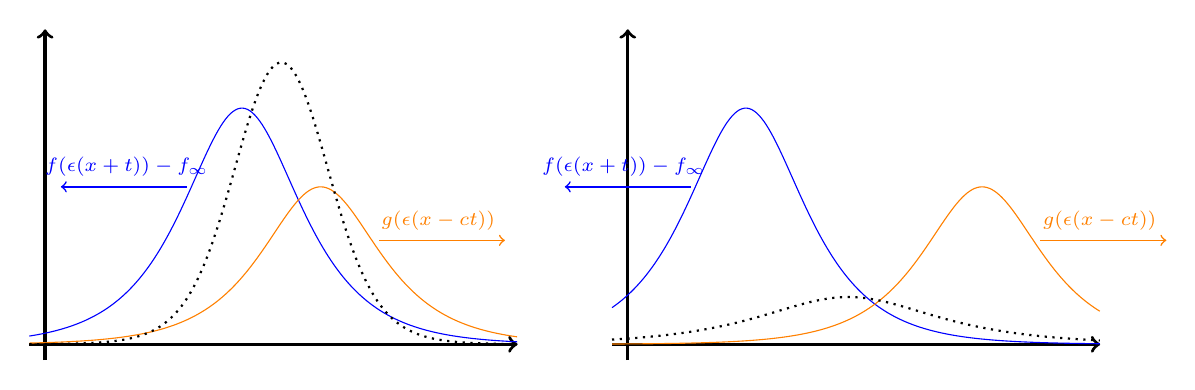
\begin{tikzpicture}[
		scale=2,
		declare function={sech(\x) = 2/(exp(\x) + exp(-\x));
			fun1(\x,\c) = 1.5 * sech((\x-\c)*3;
			fun2(\x,\c) = sech((\x-\c)*3);
		},
		]
		%axis
		\draw[->, very thick] (-0.1,0) -- (3,0) {};
		\draw[->, very thick] (0,-0.1) -- (0,2) {};
		
		%functions
		\draw[domain=-.1:3, samples = 200, color=blue] plot (\x, {fun1(\x, 1.25)} );
		\draw[domain=-.1:3, samples = 200, color=orange] plot (\x, {fun2(\x, 1.75)} );
		\draw[domain=-.1:3, samples = 200, thick, dotted] plot (\x, {2* fun1(\x,1.25) * fun2(\x,1.75)});
		
		%arrows
		\draw[->,line width=0.20mm,color=blue] (.9, 1) -- (0.1,1) {} node[above right] {\scriptsize\hspace{-1.5em} $f(\epsilon(x+t)) - f_\infty$};
		\draw[->,line width=0.20mm,color=orange] (2.12, .66) -- (2.92,.66) {} node[above left] {\scriptsize $g(\epsilon(x-ct))$};
		
		\begin{scope}[xshift=3.7cm]
			%axis
			\draw[->, very thick] (-0.1,0) -- (3,0) {};
			\draw[->, very thick] (0,-0.1) -- (0,2) {};
			
			%functions
			\draw[domain=-.1:3, samples = 200, color=blue] plot (\x, {fun1(\x, .75)} );
			\draw[domain=-.1:3, samples = 200, color=orange] plot (\x, {fun2(\x, 2.25)} );
			\draw[domain=-.1:3, samples = 200, thick, dotted] plot (\x, {0.3 * sech((\x - 1.4)*2});
			
			%arrows
			\draw[->,line width=0.20mm,color=blue] (.4, 1) -- (-0.4,1) {} node[above] {\scriptsize \hspace{5em} $f(\epsilon(x+t)) - f_\infty$};
			\draw[->,line width=0.20mm,color=orange] (2.62, .66) -- (3.42,.66) {} node[above left] {\scriptsize $g(\epsilon(x-ct))$};
		\end{scope}
	\end{tikzpicture}
	\caption{\label{fig-counter-propogating-interaction} The function \(f(\epsilon(x+t)) -f_\infty\) (shown in blue) moves to the left while \(g(\epsilon(x-ct))\) (shown in orange) moves to the right. Since they are localized, the product (shown by the dotted line) will quickly decay in time.}
\end{figure}

A suitable choice of space for \(g\) is the weighted Sobolev spaces \(H^k_n(\R)\). Here, \(H^k_n\) for \(k,n\in\mathbb N\cup \{0\}\)
\begin{equation}
	H^k_n(\R) := \{ g\in H^k(\R) \mid   g\langle \cdot \rangle^n \in H^k \}
\end{equation}
where \(\langle x \rangle = \sqrt{1+x^2}\). The norm on this space is
\begin{equation}
	\| g \|_{H^k_n(\R)} := \|  g \langle \cdot \rangle^n\|_{H^k(\R)}.
\end{equation}
This space has the useful property that if \(g \in H^k_n\), then its Fourier transform, \(\hat g \), is in \(H^n_k\) and 
\begin{equation}
	c \| \hat g \|_{H^n_k} \leq \| g \|_{H^k_n} \leq C \| \hat g \|_{H^n_k}
\end{equation}
for \(c,C>0\) independent of \(g\).

We want an analogous space for \(f\), but allowing for non-zero limits at infinity. Let \(\langle\cdot \rangle_+ :\R \to \R\) be a smooth function such that
\begin{equation}
	\langle x \rangle_+ = \begin{cases} \langle x \rangle, & x>1 \\ 1, & x<0\end{cases}
\end{equation}
and \(\langle \cdot \rangle_+\) continued smoothly between \(0\) and \(1\) such that it is always greater than or equal to \(1\). Thus \(\langle \cdot \rangle_+\) is a function that only acts like \(\langle \cdot \rangle\) for numbers greater than \(1\). The function \(\langle \cdot \rangle_-\) is similarly defined but for numbers less than \(-1\).

\begin{defn}
	Define \(\mcX^k_{n^+} (\R)\) to be the Banach space of functions where 
	\begin{equation}
		\mcX^k_{n^+} (\R) := \{ f \in \mcX^k(\R) \mid \lim_{x\to\infty} f(x) = f_\infty\text{ and } (f-f_\infty)\langle\cdot\rangle_+^n \in \mcX^k(\R)\}
	\end{equation}
	with norm given by
	\begin{equation}
		\| f \|_{\mcX^k_{n^+}(\R)} := |f_\infty| + \|(f-f_\infty) \langle \cdot \rangle_+^n \|_{\mathcal X^k(\R)}
	\end{equation}
	Similarly, 
	\begin{equation}
		\mcX^k_{n^-} (\R) := \{ f \in \mcX^k(\R) \mid \lim_{x\to-\infty} f(x) = f_{-\infty}\text{ and } (f-f_{-\infty})\langle\cdot\rangle_-^n \in \mcX^k(\R)\}
	\end{equation}
	and 
	\begin{equation}
		\| f \|_{\mcX^k_{n^-}(\R)} := |f_{-\infty}| + \|(f-f_{-\infty}) \langle \cdot \rangle_-^n \|_{\mathcal X^k(\R)}
	\end{equation}
	Define \(\mcX^k_n(\R)\) to be the intersection of these Banach spaces. That is,
	\begin{equation}
		\mcX^k_n(\R) := \mcX^k_{n^+} (\R) \cap \mcX^k_{n^-} (\R), \quad \| f \|_{\mcX^k_{n} (\R)} := \|f\|_{\mcX^k_{n^+} (\R)} + \|f\|_{\mcX^k_{n^-} (\R)}.
	\end{equation}
\end{defn}
	That \(\mcX^k_{n^\pm}\) are Banach spaces follows from the fact that there exists a linear isomorphism between the Banach space \(\R\times \mcX^k\) and these spaces, which is given by
\begin{equation}
	(\alpha, f) \mapsto \alpha + f \langle \cdot \rangle^{-n}_{\pm}.
\end{equation}
One can show that the kink solutions as specified in \cref{kink-solutions} lie in \(\mcX^k_n\) for all \(k,n\geq 0\); the derivatives are smooth and decay exponentially to zero, and the kink solutions approach the limits \(\mp\sqrt{12v}\) exponentially fast. These spaces also contain bounded rational functions. For instance, the function \[1 + \frac 1 {x^2 +1}\] is in \(\mcX^k_2(\R)\) since it approaches its limit at infinity (which in this case is \(1\)) at a rate of \(\mathcal O(1/x^2)\), and its derivatives are in \(H^0_2(\R)\).

The definitions above are used to prove that \(\phi\) remains bounded for all time. The idea behind the proof is similar to that of \cite[Lemma~3.1]{schneider2000counter}. The following lemma will be useful in showing the decay in products of \(f-f_\infty\) and \(g\).
\begin{restatable}{lem}{cknormbound}
	For each \(k\geq 0\) and \(c > 0\), there exists \(C> 0\) depending only on \(k\) such that 
	\begin{equation}\label{Ck-bound}
		\left \| \frac 1 {\langle \cdot +\tau\rangle_+^2 \langle \cdot - c\tau \rangle^2} \right \|_{C^k} \leq C\, \sup_{x\in\mathbb R} \frac 1 {\langle x +\tau\rangle_+^2 \langle x -c \tau \rangle^2}.
	\end{equation}
	Furthermore,
	\begin{equation}\label{sup-integrable}
		\int_0^\infty \sup_{x\in\mathbb R} \frac 1 {\langle x +\tau\rangle_+^2 \langle x -c \tau \rangle^2}\, d\tau <\infty.
	\end{equation}
\end{restatable}
See \cref{lemma-appendix} for proof. 

We are now ready to prove that \(\phi\) (and its time derivative) remain uniformly bounded in time.
\begin{prop}
	Fix \(T_0> 0\) and suppose that \(f \in C([-T_0,T_0], \mcX_2^{k+1}(\R))\) and \(g \in C([-T_0,T_0], H^{k+1}_2(\R)) \), with \(k>2\) an integer. Also, suppose that \(f(X,T)\to f_\infty\) as \(X\to \infty\) for any \(T\in[-T_0,T_0]\). Then there exists a constant \(C>0\) such that 
	\begin{equation}\label{phi-bound}
		\sup_{t\in[-\epsilon^{-3}T_0,\epsilon^{-3}T_0]} \|\phi(\cdot,\epsilon t)\|_{H^k} \leq C \Bigg( \sup_{t\in[-\epsilon^{-3}T_0,\epsilon^{-3}T_0]} \left\{\| f(\cdot, \epsilon^3t) \|_{\mathcal X^{k+1}_{2}},  \| g(\cdot, \epsilon^3t) \|_{H^{k+1}_2} \right\}\Bigg)^3
	\end{equation}
	and
	\begin{equation}\label{psi-bound}
		\sup_{t\in[-\epsilon^{-3}T_0,\epsilon^{-3}T_0]} \|\psi(\cdot,\epsilon t)\|_{H^{k-1}} \leq C \Bigg( \sup_{t\in[-\epsilon^{-3}T_0,\epsilon^{-3}T_0]} \left\{\| f(\cdot, \epsilon^3t) \|_{\mathcal X^{k+1}_{2}},  \| g(\cdot, \epsilon^3t) \|_{H^{k+1}_2} \right\}\Bigg)^3,
	\end{equation}
	where \(\psi = \partial_2 \phi\).
\end{prop}

\begin{proof}
	Set \(\partial_2 \phi = \psi\). Taking the Fourier transform \(\mathcal F\) on both sides of \cref{phi-pde} and writing the ODE as a first order system, we get that 
	\begin{equation}
	\begin{aligned}
		&\partial_2 \begin{bmatrix} \hat \phi(k,\tau) \\ \hat \psi(k,\tau) \end{bmatrix} = \begin{bmatrix}\hat \psi(k,\tau) \\ -k^2 \hat\phi(k,\tau) \end{bmatrix} \\ &+ \begin{bmatrix}
			0 \\   \frac 1 2 k^2 \mathcal F[ (f^2(\cdot+\tau),\epsilon^2\tau)-f_\infty^2)g(\cdot-c\tau,\epsilon^2\tau) +(f(\cdot+\tau,\epsilon^2\tau)-f_\infty)g^2(\cdot-c\tau,\epsilon^2\tau)](k)
		\end{bmatrix}.
	\end{aligned}
	\end{equation}
	The semigroup generated by the linear part can be computed explicitly. Putting the solution into variation of constants form with initial conditions set to zero gives
	\begin{equation}
	\begin{aligned}
		&\hat  \phi(k,T) = \frac 1 2 \int_0^Tk\sin(k(T-\tau)) \times\\
		&\quad\mathcal F[ (f^2(\cdot+\tau),\epsilon^2\tau)-f_\infty^2)g(\cdot-c\tau,\epsilon^2\tau) +(f(\cdot+\tau,\epsilon^2\tau)-f_\infty)g^2(\cdot-c\tau,\epsilon^2\tau)](k)\, d\tau
	\end{aligned}
	\end{equation}
	and 
	\begin{equation}\label{psi-fourier-transform}
	\begin{aligned}
		&\hat  \psi(k,T) = \frac 1 2 \int_0^Tk^2\cos(k(T-\tau)) \times\\
		&\quad\mathcal F[ (f^2(\cdot+\tau,\epsilon^2\tau)-f_\infty^2)g(\cdot-c\tau,\epsilon^2\tau) +(f(\cdot+\tau,\epsilon^2\tau)-f_\infty)g^2(\cdot-c\tau,\epsilon^2\tau)](k)\, d\tau
	\end{aligned}
	\end{equation}
	Hence we can get that 
	\begin{equation}\label{phi-sobolev-bound}
	\begin{aligned}
		&\|\phi(\cdot, T) \|_{H^k} \\
		&\quad\leq C \| \hat\phi(\cdot, T) \|_{H^0_k} \\
		&\quad\leq C \int_0^T \| \partial_1 ((f^2(\cdot+\tau)-f_\infty^2)g(\cdot-c\tau)) \|_{H^k} + \| \partial_1( (f(\cdot+\tau)-f_\infty)g^2(\cdot-c\tau)) \|_{H^k} \, \mathrm d \tau \\
		&\quad\leq C \int_0^T \| f(\cdot+\tau)\partial_1 f(\cdot + \tau)g(\cdot-c\tau) \|_{H^k} + \|(f^2(\cdot+\tau) -f_\infty^2) \partial_1 g(\cdot - c\tau) \|_{H^k}  \\
		&\qquad + \|\partial_1f(\cdot+\tau) g^2(\cdot - c\tau) \|_{H^k} + \| (f(\cdot + \tau) -f_\infty) \partial_1 g(\cdot - c\tau) \|_{H^k}\, \mathrm{d}\tau \\ 
		&\quad\leq C \int_0^T \sup_{x\in\R} \frac 1 {\langle x + \tau\rangle_+^2 \langle x - c\tau\rangle^2} \times \Bigg( \|f\|^2_{\mathcal X^{k+1}_{2}} \| g \|_{H^{k+1}_2} + \|f\|_{\mathcal X^{k+1}_{2}} \| g \|^2_{H^{k+1}_2} \Bigg) \, \mathrm d \tau, 
	\end{aligned}
	\end{equation}
	whence \cref{phi-bound} follows. The proof for \cref{psi-bound} is analogous.
\end{proof}

\section{Setup of Lattice Equations}

The scalar second-order differential equation \cref{fput-lattice-equations-strain-variables} with potential \(V\) given by \cref{truncated-potential} can be rewritten as the following first-order system:
\begin{equation}\label{first-order-lattice-eqns}
	\left\{\begin{aligned}\dot u _n &= q_{n+1} - q_n, \\
	\dot q_n &= u_n - u_{n-1} - \frac{1} 6 ( u_n^3 - u^3_{n-1}),\end{aligned} \right. \quad n \in \Z.
\end{equation}

Recall that \(u_{n} = x_{n+1} - x_n\), so we have that \(u_n\) physically represents the displacement between two neighbors on the lattice and \(q_n\) is equal to 
\begin{equation}
	q_n(t) = \sum_{k=-\infty}^{n-1} \dot u_k(t) = \sum_{k=-\infty}^{n-1} [\dot x_{k+1}(t) - \dot x_k(t)] = \dot x_n(t)
\end{equation}
and so represents the velocity at a lattice point (assuming that \(\dot x_k(t) \to 0\) as \(k\to-\infty\)). Note that we have the flexibility to add or subtract a constant from \(q\) without changing the dynamics on \(u\) (a fact that we use later to adjust the approximation and guarantee the error terms are in \(\ell^2(\Z)\)). Writing the equations for the FPUT lattice in the form given by \cref{first-order-lattice-eqns} also puts the system into a Hamiltonian framework (when \(u, q\in\ell^2(\Z)\)). Here the equations are of the form
\begin{equation}
	\dot U = J \mcH'(U)
\end{equation}
where \(U = (u,q)\), \(J\) is the skew-symmetric operator given by
\begin{equation}
	J = \begin{bmatrix}
		0 & e^\partial - 1 \\ 1 - e^{-\partial} & 0
	\end{bmatrix}
\end{equation}
and \(\mcH(U) = \sum_{n\in\Z} \frac 1 2 q_n^2 + V(u_n)\). The operators \(e^\partial\) and \(e^{-\partial}\) are the forward and backward shift operators, respectively. So we have \((e^\partial u)_n = u_{n+1}\) and \((e^{-\partial}u)_n = u_{n-1}\).

We will now introduce the traveling wave ansatz for the system in \cref{first-order-lattice-eqns}, but we first must assume certain regularity and decay of \(f\) and \(g\).
\begin{assum}\label{assumption-1}
	Let \(f\) and \(g\) be solutions of \cref{f-mKdV,g-gKdV}, respectively. Assume that \[f\in C([-\tau_0, \tau_0], \mcX_2^6(\R)) \quad \text{ and } \quad g\in C([-\tau_0,\tau_0],H_2^6(\R))\] for some \(\tau_0>0\) fixed. Furthermore, assume that \(f\) has fixed limits in its spatial variable at \(\pm \infty\) given by \(f_{\pm \infty}\).
\end{assum}

The traveling wave ansatz for \(u_n\) and \(q_n\) is then given by
\begin{equation}\label{u-ansatz}
	u_n(t) = \epsilon f(\epsilon(n+t), \epsilon^3t) + \epsilon g(\epsilon(n-ct), \epsilon^3 t) + \epsilon^3 \phi(\epsilon n , \epsilon t) + \mcU_n(t)
\end{equation}
and 
\begin{equation}\label{q-ansatz}
	q_n(t) = \epsilon F(\epsilon(n+t), \epsilon^3 t) + \epsilon G(\epsilon(n-ct), \epsilon^3 t) + \epsilon^3 \Phi(\epsilon n, \epsilon t) - \epsilon F_{-\infty} + \mcQ_n(t).
\end{equation}
The wave speed \(c\) is again given by \cref{ansatz-wave-speed}. 

The form that the ansatz takes for \(u_n(t)\) is clear. For \(q_n(t)\) we need to define \(F\), \(G\), and \(\Phi\) (where \(F_{-\infty}\) is a constant to specified shortly thereafter). One would expect  
\begin{equation}
	\begin{aligned}
		q_n(t) &= \sum_{k=-\infty}^{n-1} \dot u_n(t) \\
		&\approx \sum_{k=-\infty}^{n-1} [ \epsilon^2 \partial_1 f (\epsilon(k+t) ) + \epsilon^4 \partial_2 f(\epsilon(k+t)) \\
		&\quad+ \epsilon^2 c \partial_1 g(\epsilon (k-ct))  +\epsilon^4 \partial_2 g(\epsilon(k-ct)) \\
		&\quad+ \epsilon^4 \partial_2 \phi(\epsilon k) ].
	\end{aligned}
\end{equation}
However, the final summation does not have a simple closed form, and so would be difficult to use. Instead, the summation is approximated with simpler terms up to an appropriate order of \(\epsilon\). We choose \(F\), \(G\), and \(\Phi\) so that 
\begin{equation}
	\begin{aligned}
		\epsilon F(\epsilon (n+1 + t)) - \epsilon F(\epsilon(n+t)) &= \epsilon^2 \partial_1 f(\epsilon(n+t)) + \epsilon^4 \partial_2 f(\epsilon (n+1)) + \mathcal O(\epsilon^6) \\
		\epsilon G(\epsilon(n+1 -ct)) - \epsilon G(\epsilon(n-ct)) &=  \epsilon^2 c \partial_1 g(\epsilon (n-ct))  +\epsilon^4 \partial_2 g(\epsilon(n-ct)) + \mathcal O(\epsilon^6) \\
		\epsilon^3 \Phi(\epsilon(n+1)) - \epsilon^3 \Phi(\epsilon(n)) &= \epsilon^4 \partial_2 \phi(\epsilon n) + \mathcal O(\epsilon^6) .
	\end{aligned}
\end{equation}
After this choice, the summation of the terms on the left has a simpler and explicit representation. Thus, following some calculations, we get the following:
\begin{align}
	F &:= f - \frac{\epsilon} 2 \partial_1 f + \frac{\epsilon^2} 8 \partial_1^2 f - \frac{\epsilon^2}{12} f^3  - \frac{\epsilon^3}{48} \partial_1^3 f + \frac{\epsilon^3} 8 f^2 \partial_1 f\\
	G &:= - g + \frac{\epsilon}{2}\partial_1 g + \frac{\epsilon^2 f_\infty^2} 4  g + \frac{\epsilon^2}{12}(g^3 + 3f_\infty g^2) -\frac{ \epsilon^2} 8 \partial_1^2 g  + \frac{\epsilon^3}{48} \partial_1^3 g \\
	&\qquad - \frac{\epsilon^3}{24} \partial_1(g^3 + 3f_\infty g^2) - \frac{\epsilon^3 f_\infty^2} 8 \partial_1 g \nonumber \\
	\Phi &:=  \partial_1^{-1}\psi - \frac{\epsilon} 2 \psi.
\end{align}
Here \(\psi = \partial_2 \phi\) and \(\partial_1^{-1}\) is defined as a Fourier multiplier. That \(\partial_1^{-1}\psi\) is well-defined and in \(H^5(\R)\) follows from \cref{psi-fourier-transform}. Namely, we have that 
\begin{equation}
\begin{aligned}
	&\mcF[\partial_1^{-1} \psi(\cdot, T)](k) = (ik)^{-1} \hat\psi(k,T) \\
	&\quad = \frac{-i} 2 \int_0^T k \cos(k(T-\tau)) \times \\ &\quad \mcF[(f^2(\cdot+\tau,\epsilon^2\tau)-f_\infty^2)g(\cdot-c\tau,\epsilon^2\tau) +(f(\cdot+\tau,\epsilon^2\tau)-f_\infty)g^2(\cdot-c\tau,\epsilon^2\tau)](k) \, d\tau
\end{aligned}
\end{equation}
and (following the same calculations in \cref{phi-sobolev-bound}) 
\begin{equation}
	\| \partial_1^{-1}\psi(\cdot,T) \|_{H^5} \leq C \int_0^T \sup_{x\in\R} \frac 1 {\langle x + \tau\rangle_+^2 \langle x - c\tau\rangle^2} \times \Bigg( \|f\|^2_{\mathcal X^{6}_{2}} \| g \|_{H^{6}_2} + \|f\|_{\mathcal X^{6}_{2}} \| g \|^2_{H^{6}_2} \Bigg) \, \mathrm d \tau. 
\end{equation}\Cref{assumption-1} implies that \(F\) has fixed limits in its spatial variable at \(\pm \infty\) given by \(F_{\pm\infty} = f_{\pm\infty} -\frac{\epsilon^2}{12} f^3_{\pm\infty}\).

We want \(\mcU(t)\) and \(\mcQ(t)\) to be elements of \(\ell^2(\Z)\) (at least locally in time). However, to satisfy \(\mcQ(0)\in\ell^2(\Z)\) and \(\dot u_n(0) = q_{n+1}(0) - q_n(0)\), a compatibility condition must hold.
\begin{assum}\label{assumption-2}
	Assume that \[\sum_{n=-\infty}^\infty \dot u_n(0) = \epsilon F_{+\infty} - \epsilon F_{-\infty}.\]
\end{assum}
Note that if this did not hold, then \(\mcQ_n(0)\not\to 0\) as \(n\to\infty\) and \(\mcQ(0)\notin \ell^2(\Z)\). That \(\mcQ_n(0) \to 0\) as \(n\to-\infty\) follows directly from the ansatz. The introduction of the constant \(\epsilon F_{-\infty}\) in \cref{q-ansatz} does not affect the dynamics of \(q\) in \cref{first-order-lattice-eqns}

An equivalent set of equations to \cref{first-order-lattice-eqns} are given by
\begin{equation}\label{error-lattice-eqns}
	\left\{\begin{aligned}
			\dot{\mathcal U}_n(t) =& \, \mathcal Q_{n+1}(t) - \mathcal Q_n(t) +\ResnI \\
\dot{\mathcal Q}_n(t) =& \, \mathcal U_n(t) - \mathcal U_{n-1}(t)  \\
&\quad - \frac 1 2 (\epsilon f(\epsilon(n+t)) + \epsilon g(\epsilon(n-ct)) + \epsilon^3\phi(\epsilon n))^2 \mathcal U_{n}(t) \\
&\quad + \frac 12  (\epsilon f(\epsilon(n-1+t)) + \epsilon g(\epsilon(n-1-ct)) + \epsilon^3\phi(\epsilon (n-1)))^2 \mathcal U_{n-1}(t) \\
&\quad +\ResnII + \mathcal B_n(\epsilon f + \epsilon g + \epsilon^3 \phi,  \mathcal U) 
	\end{aligned} \right. \hspace{-0.5em}n\in\Z,
\end{equation}
where
\begin{equation}
\begin{aligned}
	\ResnI =& \epsilon F(\epsilon(n+1+t)) - \epsilon F(\epsilon(n+t)) \\
	&\quad + \epsilon G(\epsilon(n+1-c t) - \epsilon G(\epsilon(n-c t) + \epsilon^3 \Phi(\epsilon (n+1))   - \epsilon^3 \Phi(\epsilon n) \\
	&\quad - \epsilon^2 \partial_1 f(\epsilon(n+t)) - \epsilon^4 \partial_2
	f(\epsilon(n+t)) \\
	&\quad + \epsilon^2 c \partial_1 g(\epsilon(n-ct)) - \epsilon^4 \partial_2 g(\epsilon(n-ct)) - \epsilon^4 \partial_2 \phi(\epsilon n) ,
\end{aligned}
\end{equation}
\begin{equation}
\begin{aligned}
	\ResnII =& \epsilon f(\epsilon(n+t)) - \epsilon f(\epsilon(n-1+t)) \\
	&\quad+ \epsilon g(\epsilon(n-c t)) - \epsilon g(\epsilon(n-1-c t) + \epsilon^3 \phi(\epsilon n) - \epsilon^3 \phi(\epsilon (n-1)) \\
	&\quad - \epsilon^2 \partial_1 F(\epsilon(n+t)) - \epsilon^4 \partial_2
	F(\epsilon(n+t)) \\
	&\quad + \epsilon^2 c \partial_1 G(\epsilon(n-ct)) - \epsilon^4 \partial_2 G(\epsilon(n-ct)) - \epsilon^4 \partial_2 \Phi(\epsilon n) \\
	&\quad - \frac 1 6 \Big( (\epsilon f(\epsilon(n+t)) + \epsilon g(\epsilon(n-c t)) + \epsilon^3 \phi(\epsilon n))^3 \\
	&\hspace{6em} - (\epsilon f(\epsilon(n-1+t)) + \epsilon g(\epsilon(n-1-c t)) + \epsilon^3 \phi(\epsilon (n-1)))^3 \Big),
\end{aligned}
\end{equation}
and 
\begin{equation}
\begin{aligned}
	&\mathcal B_n(\epsilon f + \epsilon g + \epsilon^3 \phi, \mathcal U) \\
	&\quad= -\frac 1 6 \Big( 3(\epsilon f(\epsilon(n+t) + \epsilon g(\epsilon(n-ct)) + \epsilon^3 \phi(\epsilon n))  \mathcal U^2_n(t) \\
	&\quad \qquad - 3(\epsilon f(\epsilon(n-1+t) + \epsilon g(\epsilon(n-1-ct)) + \epsilon^3 \phi(\epsilon (n-1)))  \mathcal U^2_{n-1}(t) \\
	&\quad\qquad + \mathcal U_n^3(t)  - \mathcal U_{n-1}^3(t)\Big).
\end{aligned}
\end{equation}
The terms \(\mcU\) and \(\mcQ\) control the error associated with the ansatz in \cref{u-ansatz,q-ansatz}. Thus if these terms remain small in the \(\ell^2(\Z)\) norm, then the traveling wave ansatz will remain valid. In particular, if one has that \(\|\mcU\|_{\ell^2} \leq C\epsilon^{5/2}\), then the ansatz \(\epsilon f + \epsilon g\) is valid up to order \(\epsilon^{5/2}\) (since \(\phi\) is uniformly bounded in norm and is thus \(\mathcal O (1)\)). Similarly, if \(\mcQ\) is of order \(\epsilon^{5/2}\), then one can show that \(\dot u_n(t)\) is approximated by \(\epsilon^2 \partial_1 f + \epsilon^2 \partial_1 g\) up to order \(\epsilon^{5/2}\). Hence, controlling the norms of \(\mcU\) and \(\mcQ\) is sufficient in proving the approximation holds.

\section{Preparatory Estimates}
 
To control the dynamics of \(\mcU\) and \(\mcQ\), we need estimates of the residuals and the nonlinearity. We will frequently need to bound the \(\ell^2(\Z)\) norm of a term by the \(H^1(\R)\) norm of a function. To this end the following lemma proved in \cite{dumas2014justification} is useful.
\begin{lem}\label{h1-ell2-ineq}
	There exists \(C>0\) such that for all \(X \in H^1(\R)\) and \(\epsilon \in (0,1)\), \[\|x\|_{\ell^2} \leq C \epsilon^{-1/2} \|X\|_{H^1},\] where \(x_n := X(\epsilon n)\), \(n\in \mathbb Z\).
\end{lem}


%Proof residual terms and nonlinear terms remain small
\begin{lem}\label{residual-nonlinearity-bounds}
	Let \(f\) and \(g\) be solutions of \cref{f-mKdV,g-gKdV}, respectively, such that \(f\in C([-\tau_0, \tau_0] , \mcX^6_2)\) and \(g\in C([-\tau_0,\tau_0], H^6_2)\). Let \(\tau_0 > 0\) be fixed and \(\delta>0\) be as \begin{equation}\label{delta-defn}
		\delta := \max \left\{\sup_{\tau\in[-\tau_0, \tau_0]}\|f(\cdot,\tau)\|_{\mcX^6_2},\ \sup_{\tau\in[-\tau_0, \tau_0]} \|g(\cdot, \tau)\|_{H^6_2} \right\}
	\end{equation}
 	Then there exists a \(\delta\)-independent constant \(C>0\) such that the residual and nonlinear terms satisfy
	\begin{equation}\label{res-ineq}
		\| \ResI \|_{\ell^2} + \|\ResII \|_{\ell^2} \leq C \epsilon^{11/2} (\delta + \delta^5)
	\end{equation}
	and 
	\begin{equation}\label{nonlinear-ineq}
		\| \mathcal B_n(\epsilon f + \epsilon g + \epsilon^3 \phi, \mathcal U) \|_{\ell^2} \leq C\epsilon [ (\delta+\epsilon^2\delta^3) \|\mcU\|_{\ell^2} ^2 + \|\mcU\|_{\ell^2}^3]
	\end{equation}
	for every \(t\in[-\epsilon^{-3} \tau_0, \epsilon^{-3} \tau_0]\) and \(\epsilon \in (0,1).\)
\end{lem}

\begin{proof}
	We first focus on bounding \(\ResI\). Looking at the terms in \(\ResI\) involving \(f\) and \(F\) and using Taylor expansions and \cref{f-mKdV}, we get the following:
	\begin{equation}\label{F-res1}
		\begin{aligned}
			&\epsilon F(\cdot + \epsilon) - \epsilon F - \epsilon^2 \partial_1 f - \epsilon^4 \partial_2 f = \\
			&\hspace{10em}\begin{aligned}
				&\epsilon^2 \partial_1 f + & & \frac{\epsilon^3} 2 \partial_1^2 f +& &\frac{\epsilon^4} 6 \partial_1^3 f   & + &\frac{\epsilon^5}{24} \partial_1^4 f  \\
				& & - &\frac{\epsilon^3} 2 \partial_1^2 f & - &\frac{\epsilon^4} 4 \partial_1^3 f & - & \frac{\epsilon^5} {12} \partial_1^4 f \\
				& & & & + &\frac {\epsilon^4} 8 \partial_1^3 f & + & \frac{\epsilon^5}{16} \partial_1^4 f   \\
				& & & & - &\frac {\epsilon^4} {12} \partial_1 (f^3) & - & \frac{\epsilon^5}{24} \partial_1^2(f^3)\\
				& & & & & & - & \frac{\epsilon^5}{48} \partial_1^4 f \\
				& & & & & & + & \frac{\epsilon^5}{24} \partial_1^2 (f^3) \\
				-&\epsilon^2 \partial_1 f \\
				& & & & + &\frac{\epsilon^4}{12}\partial_1(f^3) \\
				& & & & - &\frac{\epsilon^4}{24}\partial^3 f & & & + I_{f,1}(n,t),
			\end{aligned}
		\end{aligned}
	\end{equation}
	where \(I_{f,1}\) contains the integral remainder terms:
	\begin{equation}\label{If1}
	\begin{aligned}
		I_{f,1}(n,t) := \ &\frac{\epsilon^6} {24} \int_0^1 \partial_1^5 f(\epsilon(n+t+s))(1-s)^4\, ds - \frac{\epsilon^6} {12} \int_0^1 \partial_1^5 f(\epsilon(n+t+s))(1-s)^3\, ds \\
		+ & \frac{\epsilon^6} {16} \int_0^1 \partial_1^5 f(\epsilon(n+t+s))(1-s)^2\, ds -  \frac{\epsilon^6} {24} \int_0^1 \partial_1^3 (f^3)(\epsilon(n+t+s))(1-s)^2\, ds \\
		- & \frac{\epsilon^6}{48} \int_0^1 \partial_1^5f(\epsilon(n+t+s))(1-s)\, ds +  \frac{\epsilon^6}{24} \int_0^1 \partial_1^3 (f^3)(\epsilon(n+t+s)) (1-s)\, ds.
	\end{aligned}
	\end{equation}
	Note that all the terms in \cref{F-res1} cancel except \(I_{f,1}\), and so we are only left with terms of order \(\epsilon^6\). Applying \cref{h1-ell2-ineq} (and \cref{prod-rule-1-lem,prod-rule-2-lem} when needed) to the terms in \cref{If1} gives that the \(\ell^2\) norm on the left-hand side of \cref{F-res1} can be bounded by \[C(\epsilon^{11/2}(\delta + \delta^3))\] for some choice of constant \(C>0\).
	
	Doing the same Taylor expansion for the \(g\) and \(G\) gives
	\begin{equation}
		\begin{aligned}
			&\epsilon G(\cdot + \epsilon) - \epsilon G + \epsilon^2c \partial_1 g - \epsilon^4 \partial_2 g  = \\
			&\hspace{10em}\begin{aligned}
				- & \epsilon^2 \partial_1 g & -&\frac{\epsilon^3} 2 \partial_1^2 g & - &\frac{\epsilon^4} 6 \partial_1^3 g & - & \frac{\epsilon^5}{24} \partial_1^4 g \\
				& & +&\frac{\epsilon^3} 2 \partial_1^2 g & + &\frac{\epsilon^4} 4\partial_1^3 g &+ & \frac{\epsilon^5}{12} \partial_1^4 g \\
				& & & & + &\frac{\epsilon^4 f_\infty^2} 4\partial_1 g & + & \frac{\epsilon^5f_\infty^2} 8 \partial_1^2 g  \\
				& & & & + &\frac{\epsilon^4} {12}\partial_1 (g^3) & + & \frac{\epsilon^5}{24} \partial_1^2(g^3) \\
				& & & & + &\frac{\epsilon^4} {12}\partial_1 (3f_\infty g^2) & + & \frac{\epsilon^5}{24}\partial_1^2(3f_\infty g^2)  \\
				& & & & - &\frac{\epsilon^4} {8}\partial_1^3 g & - &  \frac{\epsilon^5}{16} \partial_1^4 g  \\ 
				& & & & & & + & \frac{\epsilon^5}{48} \partial_1^4 g  \\
				& & & & & & - & \frac{\epsilon^5}{24} \partial_1^2(g^3) \\
				& & & & & & - & \frac{\epsilon^5}{24} \partial_1^2(3f_\infty g^2) \\
				& & & & & & - & \frac{\epsilon^5 f_\infty ^2} 8 \partial_1^2 g  \\
				+&\epsilon^2 \partial_1g \\
				& & & & - & \frac{\epsilon^4f_\infty ^2}{4} \partial_1 g \\
				& & & & - &\frac{\epsilon^4} {12}\partial_1 (g^3) \\
				& & & & - &\frac{\epsilon^4} {12}\partial_1 (3f_\infty g^2) \\ 
				& & & & + & \frac{\epsilon^4}{24} \partial_1^3 g && &+ I_{g,1}(nt),
			\end{aligned}
		\end{aligned}
	\end{equation}
	where \(I_{g,1}\) contains the integral remainder terms.
	\begin{equation}\label{Ig1}
	\begin{aligned}
		&I_{g,1}(n,t) := \\
		-&\frac{\epsilon^6} {24} \int_0^1 \partial_1^5 g(\epsilon(n - ct + s)) (1-s)^4 \, ds +\frac{\epsilon^6} {12} \int_0^1 \partial_1^5 g(\epsilon(n - ct + s)) (1-s)^3 \, ds \\
		+&\frac{\epsilon^6 f_\infty^2} 8 \int_0^1 \partial_1^3 g(\epsilon(n - ct + s)) (1-s)^2 \, ds +\frac{\epsilon^6} {24} \int_0^1 \partial_1^3(g^3)(\epsilon(n - ct + s)) (1-s)^2 \, ds \\
		+&\frac{\epsilon^6} {24} \int_0^1 \partial_1^3(3f_\infty g^2)(\epsilon(n - ct + s)) (1-s)^2 \, ds - \frac{\epsilon^6} {16} \int_0^1 \partial_1^5g(\epsilon(n - ct + s)) (1-s)^2 \, ds \\
		+ & \frac{\epsilon^6}{48}\int_0^1 \partial_1^5 g(\epsilon(n-ct+s))(1-s)\, ds -  \frac{\epsilon^6}{24} \int_0^1 \partial_1^3(g^3)(\epsilon(n-ct+s))(1-s)\, ds \\
		- & \frac{\epsilon^6}{24} \int_0^1 \partial_1^3(3f_\infty g^2)(\epsilon(n-ct+s))(1-s)\, ds - \frac{\epsilon^6f_\infty ^2}{8} \int_0^1 \partial_1^3 g(\epsilon(n-ct+s)) (1-s) \, ds
	\end{aligned}
	\end{equation}
	All terms except those of order \(\epsilon^6\) cancel and the terms in \cref{Ig1} can be controlled by \cref{h1-ell2-ineq}. 

	
	Similarly we have
	\begin{equation}
		\epsilon^3 \Phi(\epsilon(n+1), \epsilon t) - \epsilon^3\Phi(\epsilon n , \epsilon t) - \epsilon^4 \partial_2 \phi_2(\epsilon n, \epsilon t) =  \frac{\epsilon^6} 2 \int_0^1 \partial_1^2 \psi(\epsilon(n+s),\epsilon t)(1-s)^2\, ds,
	\end{equation}
    so the \(\ell^2\) norm can also be controlled.
	
	Therefore we have 
	\begin{equation}
		\| \ResI \|_{\ell^2} \leq C \epsilon^{11/2}(\delta + \delta^3)
	\end{equation}

	The bound on \(\ResII\) can be approached similarly. Focusing on the terms with \(f\) and \(F\) in \(\ResII\), we have 
	\begin{equation}\label{F-res2}
		\begin{aligned}
			&\epsilon f(\cdot) - \epsilon f(\cdot - \epsilon) - \epsilon^2 \partial_1 F -\epsilon^4\partial_2 F - \frac{\epsilon^3} 6 (f^3(\cdot) - f^3(\cdot - \epsilon)) =\\
			&\quad \begin{aligned}
				&\epsilon^2\partial_1 f &- &\frac{\epsilon^3} 2 \partial_1 f &+ &\frac{\epsilon^4} 6 \partial_1^3f & - & \frac{\epsilon^5}{24} \partial_1^4 f\\
				-&\epsilon^2\partial_1 f & + & \frac{\epsilon^3} 2 \partial_1^2 f &+& \frac{\epsilon^4}{12} \partial_1(f^3) - \frac{\epsilon^4} 8 \partial_1^3 f & + &  \frac{\epsilon^5}{48} \partial_1^4 f - \frac{\epsilon^5}{24}\partial_1^2(f^3)\\
				&&&& -&\epsilon^4 \partial_2 f & + & \frac{\epsilon^5} 2 \partial_1 \partial_2 f\\
				&&&& -&\frac{\epsilon^4} 6 \partial_1(f^3) & + & \frac{\epsilon^5}{12} \partial_1(f^3) & &+ I_{f,2}(n,t).
			\end{aligned}
		\end{aligned}
	\end{equation}
	where the integral remainder terms and the other terms of order \(\epsilon^6\) are contained in \(I_{f,2}\):
	\begin{equation}\label{If2}
	\begin{aligned}
		I_{f,2}(n,t) := - & \frac{\epsilon^6} {24} \int_{0}^1 \partial_1^5 f (\epsilon(n+t+s))(s-1)^4\, ds \\
		+ & \frac{\epsilon^6} {12} \int_0^1 \partial_1^2(f^3)(\epsilon(n+t+s))(s-1)^2\, ds \\
		+ & \epsilon^6\partial_2\left(\frac{1} 8 \partial_1^2 f - \frac{1}{12} f^3  - \frac{\epsilon}{48} \partial_1^3 f + \frac{\epsilon} 8 f^2 \partial_1 f\right)
	\end{aligned}
	\end{equation}
	All the above terms in \cref{F-res2} cancel except for \(I_{f,2}(n,t)\). The integral terms in \cref{If2} can be controlled like before. The non-integral term can be controlled by first evaluating the derivative in time, \(\partial_2\), and replacing the terms \(\partial_2 f\) using \cref{f-mKdV}; then the terms can be controlled by \cref{h1-ell2-ineq}. Then the left-hand side of \cref{F-res2} can be bounded by a term of the form \[ C \epsilon^{11/2}(\delta + \delta^3).\]

	Taylor expanding the remaining terms in \(\ResII\) leads to 
	\begin{equation}\label{G-res2}
	\begin{aligned}
			&\epsilon^2 \partial_1 g & - & \frac{\epsilon^3} 2 \partial_1^2g & + & \frac{\epsilon^4} 6 \partial_1^3 g & - & \frac{\epsilon^5}{24} \partial_1^4 g  \\
			&&&&+&\epsilon^4 \partial_1 \phi & - & \frac{\epsilon^5} 2 \partial_1^2  \phi \\
			-&\epsilon^2\partial_1 g & + & \frac{\epsilon^3} 2 \partial_1^2 g & - & \frac{\epsilon^4} 8 \partial_1^3 g  + \frac{\epsilon^4 f_\infty^2} 4 \partial_1 g & + & \frac{\epsilon^5}{48} \partial_1^4 g \\
			&&&&+ & \frac{\epsilon^4}{12} \partial_1(g^3 + 3f_\infty g^2) & - & \frac{\epsilon^5}{24} \partial_1^2(g^3 + 3f_\infty g^2)\\
			&&&&&& - & \frac{\epsilon^5f_\infty ^2} 8 \partial_1^2 g \\
			&&&&+&\frac{\epsilon^4f_\infty ^2} 4 \partial_1g  & - & \frac{\epsilon^5f_\infty ^2} 8 \partial_1^2 g \\
			&&&& +&\epsilon^4 \partial_2 g & - & \frac{\epsilon^5} 2 \partial_1 \partial_2 g \\ 
			&&&&-&\epsilon^4 \partial_2 \partial_1^{-1} \psi & + & \frac{\epsilon^5} 2 \partial_2 \psi\\
			&&&&-&\frac{\epsilon^4} 6 \partial_1(g^3 + 3g^2 f + 3gf^2) & + & \frac{\epsilon^5}{12}\partial_1^2(g^3 + 3g^2 f + 3gf^2),
	\end{aligned}
	\end{equation} 
	where the integral remainder terms and other terms of order \(\epsilon^6\) are contained in \(I_{g,2}\):
	\begin{equation}\label{Ig2}
	\begin{aligned}
		&I_{g,2}(n,t) = \\
		- & \frac{\epsilon^6} {24} \int_{0}^1 \partial_1^5 g(\epsilon(n-s-ct))  (s-1)^4 \, ds -  \frac{\epsilon^6}2 \int_0^1 \partial_1^3 \phi(\epsilon (n-s)) (s-1)^2\, ds \\
		- & \frac{\epsilon^6 f_\infty^2}{4}\partial_1\left( \frac{f_\infty^2} 4  g + \frac{1}{12}(g^3 + 3f_\infty g^2) -\frac{ 1} 8 \partial_1^2 g  + \frac{\epsilon}{48} \partial_1^3 g - \frac{\epsilon}{24} \partial_1(g^3 + 3f_\infty g^2) - \frac{\epsilon f_\infty^2} 8 \partial_1 g\right) \\
		-&  \epsilon^6\partial_2\left( \frac{f_\infty^2} 4  g + \frac{1}{12}(g^3 + 3f_\infty g^2) -\frac{ 1} 8 \partial_1^2 g  + \frac{\epsilon}{48} \partial_1^3 g - \frac{\epsilon}{24} \partial_1(g^3 + 3f_\infty g^2) - \frac{\epsilon f_\infty^2} 8 \partial_1 g\right) \\
		+ & \frac{\epsilon^6} {12} \int_0^1 \partial_1^3(g^3(\epsilon(n-s-ct))) (s-1)^2 ds  \\
		+ & \frac{\epsilon^6} {12} \int_0^1 \partial_1^3( 3g^2(\epsilon(n-s-ct))f(\epsilon(n-s+t))) (s-1)^2\, ds \\
		+ & \frac{\epsilon^6} {12} \int_0^1 \partial_1^3 (3g(\epsilon(n-s-ct))f^2(\epsilon(n-s+t))) (s-1)^2 \, ds
	\end{aligned}
	\end{equation}
	
	%\epsilon^6\partial_2(G_2+ \epsilon G_3)
	%\frac{\epsilon^6 L^2}{4}\partial_1(G_2 + \epsilon G_3)
	The terms in \cref{G-res2} of order \(\epsilon^3\) or lower cancel out. The terms of order \(\epsilon^4\) are equal to 
	\begin{equation}\label{psi-phi-remainder}
		-\partial_2 \partial_1^{-1} \psi+ \partial_1 \phi  - \frac 1 6 \partial_1(3(f^2 - f_\infty^2) g + 3(f-f_\infty) g^2).
	\end{equation}
	Formally applying \(\partial_1\) implies that the above terms should be constant in space since \(\partial_2 \psi = \partial_2^2 \phi\) satisfies \cref{phi-pde}. However, one should be careful with this calculation due to the differences in scaling of the spatial variables: for example, \(\phi\) and \(\psi\)'s spatial variable is rescaled to \(\epsilon n\) while \(f\)'s is rescaled to \(\epsilon(n+t)\). Taking a derivative with respect to \(\xi = \epsilon x\) gives that \cref{psi-phi-remainder} must be constant. Since all the terms decay to zero at spatial infinity, \cref{psi-phi-remainder} is exactly zero.
	
	The terms of order \(\epsilon^5\) can be rewritten as
	\begin{equation}
		\frac 1 4 \partial_1( - 2 \partial_2 g - \frac 1 {12} \partial_1^3 g + \frac 1 6 (g^3 + 3f_\infty g^2)) + \frac 1 2 (\partial_2^2\phi - \partial_1^2\phi + \frac 1 6 \partial_1^2(3(f-f_\infty )g^2 + 3 (f^2-f_\infty^2)g))
	\end{equation}
	which is equal to zero since \(g\) and \(\phi\) satisfy the PDEs in \cref{g-gKdV,phi-pde}. Thus the right-hand side of \cref{G-res2} is equal to \(I_{g,2}\). The integral terms in \cref{Ig2} are bounded as before. The remaining terms in \cref{Ig2} can be bounded by evaluating \(\partial_2 g\) using \cref{g-gKdV} and then applying \cref{h1-ell2-ineq}. We can the get the following bound: \[\| \mathrm{Res}^{(2)}(t) \|_{\ell^2} \leq C \epsilon^{11/2} (\delta + \delta^3 + \delta^5).\] Interpolating between powers of \(\delta\) gives the desired inequality \cref{res-ineq}.
	
	The proof of \cref{nonlinear-ineq} follows immediately.
\end{proof}

To proceed, we construct and energy function for \cref{error-lattice-eqns} to control the \(\ell^2\) norms of \(\mcU\) and \(\mcQ\). \Cref{residual-nonlinearity-bounds} essentially states that \(\ResI\), \(\ResII\), and \(\mathcal B\) remain appropriately small. If one drops the residual and nonlinear terms from \cref{error-lattice-eqns}, then we are left with a linear (non-autonomous) Hamiltonian system. Hence, an appropriate choice of an energy function would simply be the Hamiltonian for this reduced system (as suggested in our earlier proof sketch). Define 
\begin{equation}\label{energy-function}
	\mcE(t) = \frac 1 2 \sum_{n\in \mathbb Z} \mathcal Q_n^2(t) + \mathcal U_n^2(t) - \frac 1 2 \left(\epsilon f(\epsilon(n+t), \epsilon^3 t) + \epsilon g(\epsilon(n-ct, \epsilon^3t) + \epsilon^3 \phi(\epsilon n, \epsilon t)\right)^2 \mathcal U_n^2(t)
\end{equation}
The following lemma gives us that \(\mcE\) can be used to control \(\mcU\) and \(\mcQ\).
\begin{lem}\label{energy-coercive-bounds-lem}
	Fix \(\tau_0>0 \) and let \(\delta\) be given by \cref{delta-defn} . There exists \(\epsilon_0 = \epsilon_0(\delta) >0\) sufficiently small such that for every \(\epsilon \in (0,\epsilon_0)\) and for every local solution \((\mathcal U, \mathcal Q) \in C^1([-\tau_0\epsilon^{-3}, \tau_0\epsilon^{-3}], \ell^2(\mathbb Z))\) of \cref{error-lattice-eqns}, the energy-type quantity given in \cref{energy-function} is coercive with the bound
	\begin{equation}\label{coercive-bound}
		\|\mathcal Q(t) \|_{\ell^2}^2 + \| \mathcal U (t) \|_{\ell^2}^2 \leq  4 \mathcal E(t), \quad \text{for } t\in(-\tau_0\epsilon^{-3}, \tau_0\epsilon^{-3}).
	\end{equation}
	Moreover, there exists \(C> 0\) independent of \(\epsilon\) and \(\delta\) such that 
	\begin{equation}
		\left|\frac{d\mathcal E}{dt} \right| \leq C \mathcal E^{1/2}\left[ \epsilon^{11/2} (\delta + \delta^5)  + \epsilon^3\delta^2\mathcal E^{1/2} + \epsilon(\delta + \mathcal{E}^{1/2})\mathcal E\right]
	\end{equation}
	for every \(t\in [-\tau_0\epsilon^{-3}, \tau_0\epsilon^{-3}]\) and \(\epsilon \in (0,\epsilon_0)\). 	  
\end{lem}
\begin{proof}
	Note that \(\delta>0\) can be used to control the \(L^\infty(\R)\) norms of \(f\), \(g\), and \(\psi\). Thus we can choose \(\epsilon_0\) small enough so that for \(\epsilon \in (0,\epsilon_0)\) we have 
	\begin{equation}
		1 - \frac 12 \left( \epsilon \| f\|_{L^\infty} + \epsilon \|g\|_{L^\infty} + \epsilon^3 \| \phi \|_{L^\infty} \right)^2 \geq \frac 12,
	\end{equation}
	independent on the particular choices of \(f\) and \(g\). 	Hence
	\begin{equation}
		\mathcal E(t) \geq \frac 1 2 \| \mathcal Q \|_{\ell^2}^2 + \frac 1 4 \| \mathcal U\|_{\ell^2}^2 \geq \frac 1 4\| \mathcal Q \|_{\ell^2}^2 + \frac 1 4 \| \mathcal U\|_{\ell^2}^2
	\end{equation}
	and \cref{coercive-bound} follows.
	
	Now we take the time derivative of \(\mathcal E\) to get that 
	\begin{equation}
	\begin{aligned}
		\frac{d\mcE}{dt} = \sum_{n \in \Z} &\mathcal Q_n(t) \ResnII + \mathcal Q_n(t) 	\mathcal B_n(\epsilon f + \epsilon g + \epsilon^3 \phi, \mathcal U(t)) \\
		&+ \mathcal U_n(t) \ResnI \left( 1 - \frac 12 (\epsilon f+ \epsilon g + \epsilon^3 \phi)^2  \right) \\
		&+ \mathcal U_n^2(t)(\epsilon f + \epsilon g + \epsilon^3 \phi) \times (\epsilon^2\partial_1 f + \epsilon^4\partial_2 f -\epsilon^2 c \partial_1 g + \epsilon^4 \partial_2 g + \epsilon^4 \partial_2 \phi).
	\end{aligned}
	\end{equation}
	Then using the Cauchy inequality and the H\"older inequality for \(p=1\) and \(q=\infty\) we get that
	\begin{equation}
	\begin{aligned}
		\left| \frac{d\mathcal E}{dt} \right| \leq& \| \mathcal Q \|_{\ell^2 }\times \|\ResII \|_{\ell^2} + \| \mathcal Q \|_{\ell^2} \times \| \mathcal B \|_{\ell^2}  + \|\mathcal U \|_{\ell^2} \times \| \ResnI \|_{\ell^2}\\
		& + \|\mathcal U^2 \|_{\ell^1} \times  \| (\epsilon f+ \epsilon g + \epsilon^3 \phi)  \times  (\epsilon^2\partial_1 f + \epsilon^4\partial_2 f -\epsilon^2 c \partial_1 g + \epsilon^4 \partial_2 g + \epsilon^4 \partial_2 \phi )\|_{\ell^\infty} .
	\end{aligned}
	\end{equation}
	Note that if \(a \in \ell^2\), then \(a\in \ell^\infty\) and \(\|a\|_{\ell^\infty} \leq \|a \|_{\ell^2}\). Thus we can replace the \(\ell^\infty\) norms above with \(\ell^2\) norms. Using the results in \cref{residual-nonlinearity-bounds}, we thus have 
	\begin{equation}
	\begin{aligned}
		\left| \frac{d\mathcal E}{dt} \right| \leq& C\Big[\mathcal E^{1/2} \epsilon^{11/2}(\delta + \delta^5) + \mathcal E^{1/2}\epsilon [(\delta + \epsilon^2 \delta^3)\mathcal E + \mathcal E^{3/2}]  \\
		&\quad + \mathcal E(\epsilon^3 \delta^2 + \epsilon^5\delta^2 + \epsilon^5 \delta^4 + \epsilon^7\delta^4 + \epsilon^7 \delta^6) \Big],
	\end{aligned}
	\end{equation}
 	where the \(C>0\) is independent of \(\epsilon\) and \(\delta\). The right-hand side of the above inequality can be simplified by taking \(\epsilon_0\) smaller. That is, taking \(\epsilon_0\) sufficiently small (dependent on \(\delta\)), we can absorb higher orders of \(\epsilon\) into lower orders. For example, \(\epsilon^3 \delta^2 + \epsilon^5\delta^2 \leq 2 \epsilon^3 \delta^2\) for \(\epsilon\) small enough. Thus we arrive at  		
	\begin{equation}
		\left|\frac{d\mathcal E}{dt} \right| \leq C \mathcal E^{1/2}\left[ \epsilon^{11/2} (\delta + \delta^5)  + \epsilon^3\delta^2\mathcal E^{1/2} + \epsilon(\delta + \mathcal{E}^{1/2})\mathcal E\right]
	\end{equation}
	as desired.
\end{proof}


Lastly, before we can prove our main result, we must show that for appropriate initial conditions that \(\mcU(0)\) and \(\mcQ(0)\) are suitably small. In particular, we want our initial conditions to be ``close to" the traveling wave ansatz in the sense that 
\begin{equation}
	u_n(0) \approx \epsilon f(\epsilon n , 0) + \epsilon g(\epsilon n , 0)
\end{equation}
and 
\begin{equation}
	\dot u_n(0) \approx \epsilon \partial_1 f(\epsilon n , 0) -\epsilon^2 g(\epsilon n,0)
\end{equation}
where the higher-order \(\epsilon\) terms are neglected. Recall that we assume \(\phi\) and \(\partial_1\phi\) to have initial conditions exactly equal to zero, so those terms drop. A seemingly appropriate notion of ``closeness" would be in the \(\ell^2\) norm, as used in \cite{khan2017long,schneider2000counter}. However, since \(q_n(0) = \sum_{k=-\infty}^{n-1} \dot u_{k}(0)\), we may lose some decay due to the summation and \(\mcQ(0)\) will not be in \(\ell^2\). To counter this, we need some extra localization assumptions on \(\dot u_n(0)\).

\begin{assum}\label{assumption-3}
	Suppose that the initial conditions for \(u\) satisfy
	\begin{equation}
		\| u(0) - \epsilon f(\epsilon \cdot, 0) - \epsilon g(\epsilon \cdot, 0) \|_{\ell^2} + \| \dot u(0) - \epsilon^2 \partial_1 f(\epsilon \cdot, 0) + \epsilon^2 \partial g (\epsilon \cdot , 0) \|_{\ell^2_2} \leq \epsilon^{5/2}
	\end{equation}
	and that \(f(\cdot, 0) \in \mcX^6_2\) and \(g(\cdot, 0) \in H^6_2\)
\end{assum}

The \(\ell^2_2\) norm will be sufficient to get that the summation is in \(\ell^2\) based on the following lemma.
\begin{restatable}{lem}{elltwo}
\label{ell22-lemma}
	If \(a\in \ell^2_2(\Z)\) and 
	\begin{equation}
		\sum_{k=-\infty}^n a_k = 0,
	\end{equation}
	then \(b_n = \sum_{k=-\infty}^n a_k\) is in \(\ell^2(\Z)\) and 
	\begin{equation}
		\|b\|_{\ell^2} \leq C \|a\|_{\ell^2_2}
	\end{equation}
	for some \(C> 0\) independent of \(a\).
\end{restatable} 
See \cref{lemma-appendix} for proof.


We can now show the following.
\begin{lem}\label{initial-conditions-lem}
	Let \cref{assumption-2,assumption-3} hold. Then \(\mcU(0),\mcQ(0) \in \ell^2(\Z)\) satisfy
	\begin{equation}\label{diff-eqn}
		\dot u_n(0) = q_{n+1}(0) - q_n(0)
	\end{equation}
	and 
	\begin{equation}\label{initial-condition-ineq}
		\| \mcU(0) \|_{\ell^2} + \|\mcQ(0)\|_{\ell^2} \leq C \epsilon^{5/2}
	\end{equation}
	with \(C>0\) independent of \(\epsilon\).
\end{lem}

\begin{proof}
	That \(\|\mcU(0)\|_{\ell^2}\leq C \epsilon^{5/2}\) follows immediately from applying \cref{assumption-3} to \cref{u-ansatz}.
	
	For \(q_n(0)\) to satisfy \cref{diff-eqn}, it must equal \(\sum_{k=-\infty}^{n-1} \dot u_k(0)\) (modulo a constant which we assume without loss of generality to be zero). Thus we have
	\begin{equation}\label{q0-summation}
	\begin{aligned}	
		q_n(0) =& \sum_{k=-\infty}^{n-1} \dot u_k(0)\\
		=& \sum_{k=-\infty}^{n-1}\left[ \dot u_k(0) - \epsilon^2 \partial_1 f(\epsilon k,0) - \epsilon^4 \partial_1 f(\epsilon k,0) + \epsilon^2 c \partial_1 g(\epsilon k,0) - \epsilon^4 \partial_2g(\epsilon k,0)\right] \\
		&+\sum_{k=-\infty}^{n-1}\left[  \epsilon^2 \partial_1 f(\epsilon k,0) +\epsilon^4 \partial_1 f(\epsilon k,0) - \epsilon F(\epsilon(k+1),0) +\epsilon F(\epsilon k ,0)  \right] \\
		&+ \sum_{k=-\infty}^{n-1}\left[ - \epsilon^2 c\partial_1 g(\epsilon k,0) +\epsilon^4 \partial_1 g(\epsilon k,0) - \epsilon G(\epsilon(k+1),0) +\epsilon G(\epsilon k ,0)  \right] \\
		&+ \epsilon F(\epsilon n, 0) - \epsilon F_{-\infty} + \epsilon G(\epsilon n, 0).
	\end{aligned}
	\end{equation}
	Comparing \cref{q0-summation} to \cref{q-ansatz}, we have that 
	 \begin{equation}\label{mcq-zero}
	 \begin{aligned}
		\mcQ_n(0) =& \sum_{k=-\infty}^{n-1}\left[ \dot u_k(0) - \epsilon^2 \partial_1 f(\epsilon k,0) - \epsilon^4 \partial_1 f(\epsilon k,0) + \epsilon^2 c \partial_1 g(\epsilon k,0) - \epsilon^4 \partial_2g(\epsilon k,0)\right] \\
		&+\sum_{k=-\infty}^{n-1}\left[  \epsilon^2 \partial_1 f(\epsilon k,0) +\epsilon^4 \partial_1 f(\epsilon k,0) - \epsilon F(\epsilon(k+1),0) +\epsilon F(\epsilon k ,0)  \right] \\
		&+ \sum_{k=-\infty}^{n-1}\left[ - \epsilon^2 c\partial_1 g(\epsilon k,0) +\epsilon^4 \partial_1 g(\epsilon k,0) - \epsilon G(\epsilon(k+1),0) +\epsilon G(\epsilon k ,0)  \right].
	\end{aligned}
	\end{equation}
	That \(\mcQ_n(0)\to 0\) as \(n\to\infty\) is guaranteed by \cref{assumption-2}. Now \cref{ell22-lemma} can be applied to get the result if the summands are in \(\ell^2_2\) and of order \(\epsilon^{5/2}\). The first summand satisfies this condition because of \cref{assumption-3}.  Note that the latter summands are equal to \(-I_{f,1}(k,0)\) and \(-I_{g,1}(k,0)\), as defined in \cref{If1,Ig1}. This follows from the earlier calculations in \cref{residual-nonlinearity-bounds}. That \(I_{f,1}(k,0)\) and \(I_{g,2}(k,0)\) are elements of \(\ell^2_2\) follows from \(f(\cdot, 0) \in \mcX^6_2\) and \(g(\cdot, 0) \in H^6_2\) and an application of \cref{h1-ell2-ineq}.
	
	Thus we have \cref{initial-condition-ineq} where the \(C>0\) can be chosen based on the norms of \(f\) and \(g\).
\end{proof}

\section{Long-time approximation of FPUT}

In this section, we prove that the solutions of the FPUT can be approximated by counter-propagating solutions for the KdV equations given in \cref{f-mKdV} and \cref{g-gKdV} for times scales of order \(\epsilon^{-3}\).

\begin{theorem}
	Let \cref{assumption-1} hold and set
	\begin{equation}
		\delta = \max \left\{\sup_{\tau\in[-\tau_0, \tau_0]}\|f(\cdot,\tau)\|_{\mcX^6_2},\ \sup_{\tau\in[-\tau_0, \tau_0]} \|g(\cdot, \tau)\|_{H^6_2} \right\}
	\end{equation}
	There exists positive constants \(\epsilon_0\) and \(C\) such that for all \(\epsilon \in(0,\epsilon_0)\), when initial data \((u(0), \dot u(0))\) satisfy \cref{assumption-2,assumption-3}, the unique solution \((u,q)\) to the FPU equation \cref{first-order-lattice-eqns} belongs to 
	\begin{equation}
		C^1([-t_0(\epsilon), t_0(\epsilon)], \ell^\infty(\mathbb Z))
	\end{equation}
	with \(t_0(\epsilon):= \epsilon^{-3}\tau_0 \) and satisfies
	\begin{equation}
		\begin{aligned}
			&\| u(t) - \epsilon f(\epsilon(\cdot+t), \epsilon^3 t) -\epsilon g(\epsilon(\cdot -ct) ,\epsilon^3 t) \|_{\ell^2} \\
			&\quad + \| \dot u(t) - \epsilon \partial_1 f(\epsilon (\cdot +t),\epsilon^3t)  +\epsilon^2 \partial_1 g(\epsilon(\cdot - ct), \epsilon^3t)\|_{\ell^2} \leq C \epsilon^{5/2 }, \quad t\in[-t_0(\epsilon), t_0(\epsilon)].
		\end{aligned}
	\end{equation}
\end{theorem}

\begin{proof}
	Set \(\mathcal S := \mathcal E ^{1/2}\) where \(\mathcal E\) is defined in \cref{energy-function}. From the results in \cref{initial-conditions-lem}, we get that \(\mathcal S(0) \leq C_0 \epsilon^{5/2}\) for some constant \(C_0 > 0\) and \(\epsilon_0\) as chosen in \cref{energy-coercive-bounds-lem}. For fixed constant \(C> 0\) define
	\begin{equation}
		T_{C} := \sup \left\{T_0 \in (0,   \epsilon^{-3} \tau_0]: \mathcal S(t) \leq C \epsilon^{5/2},\, t\in [-T_0, T_0]\right\}.
	\end{equation} 
	The goal is then to pick \(C\) so that \(T_{C} = \epsilon^{-3} \tau_0\).
	
	We have that
	\begin{equation}
		\begin{aligned}
			\left | \frac d {dt} \mathcal S(t) \right | &= \frac 1 {2 \mathcal E ^{1/2}} \left | \frac d {dt} \mathcal E(t) \right| \\
			&\leq C_1(\delta + \delta^5) \epsilon^{11/2} + C_2 \epsilon^3\left[ \delta^2 + \epsilon^{-2}(\delta + \mathcal S) \mathcal S \right]\mathcal S
		\end{aligned}
	\end{equation}
	where \(C_1, C_2 > 0\) are independent of \(\delta\) and \(\epsilon\). While \(|t| \leq T_{C}\),
	\begin{equation}
		C_2 \left[ \delta^2 + \epsilon^{-2}(\delta + \mathcal S) \mathcal S \right] \leq C_2 \left[ \delta^2  + (\delta +  C\epsilon^{5/2}) C \epsilon^{1/2} \right],
	\end{equation}
	where the right-hand side is continuous in \(\epsilon \) for \(\epsilon \in [0,\epsilon_0]\) and \(C>0\). Furthermore, the right-hand side of the inequality above is increasing in both \(\epsilon\) and \(C\), and so we can uniformly bound the term by some fixed number. Set \(K(C,\epsilon_0)= K>0\) to be
	\begin{equation}\label{K-def-2}
		K :=  \left[ \delta^2  + (\delta +  C\epsilon_0^{5/2}) C \epsilon_0^{1/2} \right].
	\end{equation}
	
	Hence, we can get that for \(t \in [-T_{C}, T_{C}]\) 
	\begin{equation}
		\begin{aligned}
			\frac d {dt} e^{-\epsilon^3 K t} \mathcal S(t) &= - \epsilon^3 K e^{-\epsilon^3 K t} \mathcal S  + e^{-\epsilon^3 K t} \frac d {dt} \mathcal S \\
			&\leq - \epsilon^3 K e^{-\epsilon^3 K t} \mathcal S  + e^{-\epsilon^3 K t}C_1(\delta + \delta^5) \epsilon^{11/2} \\
			&\qquad+ e^{-\epsilon^3 K t}C_2 \epsilon^3\left[ \delta^2 + \epsilon^{-2}(\delta + \mathcal S) \mathcal S \right]\mathcal S \\
			&\leq - \epsilon^3 K e^{-\epsilon^3 K t} \mathcal S  +  e^{-\epsilon^3 K t}C_1(\delta + \delta^5) \epsilon^{11/2} + \epsilon^3 K e^{-\epsilon^3 K t}\mathcal S \\
			&= e^{-\epsilon^3 K t}C_1(\delta + \delta^5) \epsilon^{11/2}.
		\end{aligned}
	\end{equation}
	Integrating gives
	\begin{equation} 
		\begin{aligned}
			\mathcal S(t) &\leq \left( \mathcal S(0) + K^{-1} C_1 (\delta+\delta^5) \epsilon^{5/2} \right) e^{\epsilon^3 K t} - \epsilon^{5/2} K^{-1} C_1 (\delta + \delta^5) \\
			&\leq \left(C_0+ K^{-1} C_1 (\delta+\delta^5)  \right) \epsilon^{5/2}e^{\epsilon^3 K t} \\
			&\leq (C_0 + K^{-1} C_1 (\delta+\delta^5) ) e^{K\tau_0} \epsilon^{5/2}
		\end{aligned}
	\end{equation}
	for \(t \in [-T_{C}, T_{C}]\). If we have 
	\begin{equation}\label{C-ineq-bound}
		(C_0 + K^{-1} C_1 (\delta+\delta^5) ) e^{K\tau_0}  \leq C
	\end{equation} 
	then we can conclude that \(T_C = \epsilon^{-3}\tau_0.\) Note that the left-hand side of the inequality goes to 
	\begin{equation}
		(C_0 + \delta^{-2} C_1 (\delta+\delta^5) ) e^{\delta^2\tau_0}
	\end{equation}
	as \(\epsilon \to 0\) for fixed values of \(C\). Thus choose \(C>0\) large enough so that
	\begin{equation}
		(C_0 + \delta^{-2} C_1 (\delta+\delta^5) ) e^{\delta^2\tau_0} < C
	\end{equation}
 	and then we can make \(\epsilon_0\) sufficiently small so that \cref{C-ineq-bound} holds for all \(\epsilon \in (0,\epsilon_0]\).
\end{proof}

\section{Meta-stability of kink-like solutions}

We would now like to apply a similar method as seen in \cite{khan2017long} to show that the approximations hold for time scales of order \(\epsilon^{-3}|\log(\epsilon)|\). This is a useful result because one can then make conclusions about the meta-stability of the kink-like solution on the FPUT from the stability of the kink solution for the mKdV. 

However, we cannot use the full approximation with the counter-propagating solutions. The problem comes from trying to extend \cref{assumption-1}. To make sure \(\phi\) remains bounded for longer period of times, we need to assume that \(f\) and \(g\) remain localized for longer and longer times. However, the PDEs \cref{f-mKdV} and \cref{g-gKdV} are dispersive, and so generic solutions will become less localized over time resulting in larger norms in \(\mcX^6_2\) and \(H^6_2\).

The localization assumption is only necessary to keep \(\phi\), the term coming from the coupling of \(f\) and \(g\), bounded. We can drop this assumption if we set \(g\) identically equal to zero. It is easy to see that if \(g=0\) then \(\phi = 0\). Also, one can check that the estimates of the residuals and nonlinear terms rely only on \(f \in \mcX^6\) if \(\phi = 0\), and so our estimates from before still hold in this case.

\begin{assum}\label{assumption-4}
	Let \(f\) be a solution to \cref{f-mKdV} and set \(g = 0\). Assume that 
	\begin{equation}
		f \in C_b(\R, \mcX^6(\R)).
	\end{equation}
	Furthermore, assume that \(f\) has fixed limits in its spatial variables at \(\pm \infty\) given by \(f_{\pm \infty}\).
\end{assum}

We will still need to assume that the initial condition of \(f\) is still localized as in \cref{assumption-3}, but this assumption holds for many solutions including the kink solutions of \cref{f-mKdV}.

The following result and proof are analogous to those of \cite[Thm.~1]{khan2017long}.

\begin{theorem}
	Let \cref{assumption-4} hold and set 
	\begin{equation}
		\delta =\sup_{\tau\in\R}\|f(\cdot,\tau)\|_{\mcX^6}
	\end{equation}
	For fixed \(r\in(0,1/2)\), there exists positive constants \(\epsilon_0\), \(C\), and \(K\) such that for all \(\epsilon \in(0,\epsilon_0)\), when initial data \((u(0), \dot u(0))\) satisfy \cref{assumption-2,assumption-3}, the unique solution \((u,q)\) to the FPU equation \cref{first-order-lattice-eqns} belongs to 
	\begin{equation}
		C^1([-t_0(\epsilon), t_0(\epsilon)], \ell^\infty(\mathbb Z))
	\end{equation}
	with \(t_0(\epsilon):= r K^{-1} \epsilon^{-3} | \log (\epsilon) | \) and satisfies
	\begin{equation}
	\begin{aligned}
		&\| u(t) - \epsilon f(\epsilon(\cdot+t), \epsilon^3 t) \|_{\ell^2} \\
		&\quad + \| \dot u(t) - \epsilon \partial_1 f(\epsilon (\cdot +t),\epsilon^3t)  \|_{\ell^2} \leq C \epsilon^{5/2 - r}, \quad t\in[-t_0(\epsilon), t_0(\epsilon)].
	\end{aligned}
	\end{equation}
\end{theorem}

\begin{proof}
	%Need to show local existence of solutions
	
	Set \(\mathcal S := \mathcal E ^{1/2}\) where \(\mathcal E\) is defined in \cref{energy-function}. From the results in \cref{initial-conditions-lem}, we get that \(\mathcal S(0) \leq C_0 \epsilon^{5/2}\) for some constant \(C_0 > 0\) and \(\epsilon_0\) as chosen in \cref{energy-coercive-bounds-lem}. For fixed constants \(r\in(0,1/2)\), \(C> C_0\), and \(K > 0\), define the maximal continuation time by 
	\begin{equation}
		T_{C,K,r} := \sup \left\{T_0 \in (0, r K^{-1} \epsilon^{-3} |\log(\epsilon)|]: \mathcal S(t) \leq C \epsilon^{5/2 -r}, t\in [-T_0, T_0]\right\}.
	\end{equation} 
	We also define the maximal evolution time of the mKdV equation as \(\tau_0(\epsilon) = rK^{-1}|\log(\epsilon)|\). The goal is then to pick \(C\) and \(K\) so that \(T_{C,K,r} = \epsilon^{-3} \tau_0(\epsilon)\).
	
	We have that
	\begin{equation}
	\begin{aligned}
		\left | \frac d {dt} \mathcal S(t) \right | &= \frac 1 {2 \mathcal E ^{1/2}} \left | \frac d {dt} \mathcal E(t) \right| \\
		&\leq C_1(\delta + \delta^5) \epsilon^{11/2} + C_2 \epsilon^3\left[ \delta^2 + \epsilon^{-2}(\delta + \mathcal S) \mathcal S \right]\mathcal S
	\end{aligned}
	\end{equation}
	where \(C_1, C_2 > 0\) are independent of \(\delta\) and \(\epsilon\). While \(|t| \leq T_{C,K,r}\),
	\begin{equation}
		C_2 \left[ \delta^2 + \epsilon^{-2}(\delta + \mathcal S) \mathcal S \right] \leq C_2 \left[ \delta^2  + \epsilon^{-2}(\delta +  C\epsilon^{5/2-r}) C \epsilon^{5/2-r} \right],
	\end{equation}
	where the right-hand side is continuous in \(\epsilon \) for \(\epsilon \in [0,\epsilon_0]\). Thus the right-hand side can be uniformly bounded by a constant independent of \(\epsilon\). Choose \(K>0\) (dependent on \(C\)) sufficiently large so that 
	\begin{equation}\label{K-def}
		C_2 \left[ \delta^2  + \epsilon^{-2}(\delta +  C\epsilon^{5/2-r}) C \epsilon^{5/2-r} \right] \leq K.
	\end{equation}

	Hence, we can get that for \(t \in [-T_{C,K,r}, T_{C,K,r}]\) 
	\begin{equation}
	\begin{aligned}
		\frac d {dt} e^{-\epsilon^3 K t} \mathcal S(t) &= - \epsilon^3 K e^{-\epsilon^3 K t} \mathcal S  + e^{-\epsilon^3 K t} \frac d {dt} \mathcal S \\
		&\leq - \epsilon^3 K e^{-\epsilon^3 K t} \mathcal S  + e^{-\epsilon^3 K t}C_1(\delta + \delta^5) \epsilon^{11/2} \\
		&\qquad+ e^{-\epsilon^3 K t}C_2 \epsilon^3\left[ \delta^2 + \epsilon^{-2}(\delta + \mathcal S) \mathcal S \right]\mathcal S \\
		&\leq - \epsilon^3 K e^{-\epsilon^3 K t} \mathcal S  +  e^{-\epsilon^3 K t}C_1(\delta + \delta^5) \epsilon^{11/2} + \epsilon^3 K e^{-\epsilon^3 K t}\mathcal S \\
		&= e^{-\epsilon^3 K t}C_1(\delta + \delta^5) \epsilon^{11/2}.
	\end{aligned}
	\end{equation}
	Integrating gives
	\begin{equation} 
	\begin{aligned}
		\mathcal S(t) &\leq \left( \mathcal S(0) + K^{-1} C_1 (\delta+\delta^5) \epsilon^{5/2} \right) e^{\epsilon^3 K t} - \epsilon^{5/2} K^{-1} C_1 (\delta + \delta^5) \\
		&\leq \left( \mathcal S(0) + K^{-1} C_1 (\delta+\delta^5) \epsilon^{5/2} \right) e^{\epsilon^3 K t} \\
		&\leq \left( \mathcal S(0) + K^{-1} C_1 (\delta+\delta^5) \epsilon^{5/2} \right) e^{ K \tau_0(\epsilon)} \\
		&\leq \left( C_0 + K^{-1} C_1 (\delta+\delta^5)  \right) \epsilon^{5/2 -r}
	\end{aligned}
	\end{equation}
	for \(t \in [-T_{C,K,r}, T_{C,K,r}]\), where the last line follows in part from the definition of \(\tau_0(\epsilon)\). Now choose \(C> C_0\) sufficiently large so that 
	\begin{equation}
		C_0 + K^{-1} C_1(\delta + \delta^5) \leq C.
	\end{equation}
	Note that our earlier choice of \(K\) can be enlarged so that \cref{K-def} still holds as well as the above inequality. Therefore, with these choices of \(C\) and \(K\), the maximal interval can be extended to \(T_{C,K,r} = \epsilon^{-3} \tau_0(\epsilon) \). 
\end{proof}
	\cleardoublepage

	
	\appendix
	\begin{appendices}
		% !TeX root = ../thesis.tex
\chapter{Proofs of lemmas}\label{lemma-appendix}
\prodruleone*
\begin{proof}
	The result follows from induction on \(k\).
	
	For \(k = 0\), we have
	\begin{equation}
		\| f g \|_{H^0} \leq \| f \|_{L^\infty} \| g\|_{H^0}.
	\end{equation}
	
	Assuming \cref{prod_rule} holds for \(k\geq 0\), we have that 
	\begin{align*}
		\| f g \|_{H^{k+1}} \leq C \left( \| f g \|_{H^k} + \| \partial^{k+1}(fg) \|_{L^2}\right) \\
		\leq C \left( \| f\|_{\mathcal X^k} \| g \|_{H^k} + \| \partial^{k+1}(fg) \|_{L^2} \right),
	\end{align*}
	where the second term can be bounded by 
	\begin{align*}
		\| \partial^{k+1}(fg) \|_{L^2} &\leq \| \partial^k(\partial^1 f g ) \|_{L^2} + \| \partial^k(f \partial^1 g) \|_{L^2} \\
		&\leq \| \partial^1 f  g \|_{H^k} + \| f \partial^1 g \|_{H^k} \\
		&\leq \| \partial^1 f \|_{H^k} \|g\|_{H^k} + \|f\|_{\mathcal X^k} \|\partial^1 g\|_{H^k} \\
		&\leq \| f \|_{\mathcal X^{k+1}} \| g\|_{H^{k+1}} + \|f \|_{\mathcal X^{k+1}} \|g\|_{H^{k+1}} \\
		&= 2  \| f \|_{\mathcal X^{k+1}} \| g\|_{H^{k+1}}.
	\end{align*}
	This completes the induction.
\end{proof}

\prodruletwo*
\begin{proof}
	content...
\end{proof}

\cknormbound*
\begin{proof}
	The main argument of the proof is given by showing the following claim holds:
	
	\emph{Claim}: For each integer \(k\geq 0\), \[\frac{\partial^k}{\partial x^k} \left[\frac 1 {\langle x+\tau\rangle_+^2 \langle x -c\tau \rangle^2}\right]\] is a sum of terms of the form 
	\begin{equation}\label{term}
		\frac C {\langle x +\tau\rangle_+^{2+m} \langle x -c\tau \rangle^{2+m}}\langle x + \tau \rangle_+^{m_1}\langle x-c\tau\rangle^{m_2} F(x,\tau),
	\end{equation} where \(C\neq 0\) is a constant, \(m,m_1,m_2\) are integers, \(0\leq m_1, m_2 \leq m\), and \(F\in C^n_b(\R\times\R)\) for every \(n\in \mathbb N\).
	
	This can be proved inductively. We have the \(k = 0\) case immediately by setting \(C = 1\), \(m=m_1=m_2 = 0\), and \(F(x) = 1\). Now we assume that the claim holds for \(k\geq 0\). To get the form of the \((k+1)^\text{st}\) derivative, we can use linearity and look at the derivative of each term of the form \cref{term}. That is, the \((k+1)^\text{st}\) derivative is a sum of terms of the form 
	\begin{equation}\label{term2}
		\frac{\partial}{\partial x}\left[\frac C {\langle x +\tau\rangle_+^{2+m} \langle x -c\tau \rangle^{2+m}}\langle x + \tau \rangle_+^{m_1}\langle x-c\tau\rangle^{m_2} F(x,\tau)\right].
	\end{equation}
	Applying the product rule to \cref{term2} gives us 
	\begin{align*}
		\frac{\partial}{\partial x}\Bigg[&\frac C {\langle x +\tau\rangle_+^{2+m} \langle x -c\tau \rangle^{2+m}} \langle x + \tau \rangle_+^{m_1}\langle x-c\tau\rangle^{m_2} F(x,\tau)\Bigg] = \\
		&\qquad\quad \underbrace{\frac{\partial}{\partial x}\left[\frac C {\langle x +\tau\rangle_+^{2+m} \langle x -c\tau \rangle^{2+m}}\right]\langle x + \tau \rangle_+^{m_1}\langle x-c\tau\rangle^{m_2} F(x,\tau)}_{I} \\
		&\qquad+ \underbrace{\frac C {\langle x +\tau\rangle_+^{2+m} \langle x -c\tau \rangle^{2+m}}\frac{\partial}{\partial x}\left[\langle x + \tau \rangle_+^{m_1}\right]\langle x-c\tau\rangle^{m_2} F(x,\tau)}_{II} \\
		&\qquad+ \underbrace{\frac C {\langle x +\tau\rangle_+^{2+m} \langle x -c\tau \rangle^{2+m}}\langle x + \tau \rangle_+^{m_1}\frac{\partial}{\partial x}\left[\langle x-c\tau\rangle^{m_2}\right] F(x,\tau)}_{III} \\
		&\qquad+ \underbrace{\frac C {\langle x +\tau\rangle_+^{2+m} \langle x -c\tau \rangle^{2+m}}\langle x + \tau \rangle_+^{m_1}\langle x-c\tau\rangle^{m_2} \frac{\partial}{\partial x}\left[F(x,\tau)\right] }_{IV}.
	\end{align*}
	
	We now go term-by-term. For the first term, we have
	\begin{align*}
		I =& \frac {-(2+m)C} {\langle x +\tau\rangle_+^{2+(m+1)} \langle x -c\tau \rangle^{2+(m+1)}}\langle x + \tau \rangle_+^{m_1+1}\langle x+\tau\rangle^{m_2} \Big(\langle x-c\tau\rangle_+'F(x,\tau)\Big) \\
		&\quad-\frac {(2+m)C} {\langle x +\tau\rangle_+^{2+(m+1)} \langle x -c\tau \rangle^{2+(m+1)}}\langle x + \tau \rangle_+^{m_1}\langle x-c\tau\rangle^{m_2+1} \Big(\langle x-c\tau\rangle'F(x,\tau)\Big),
	\end{align*}
	where \(\langle \cdot \rangle'\) denotes the derivative of \(\langle \cdot \rangle\). It's clear that both of these are of the form in \cref{term}.
	
	Also, we have 
	\begin{align*}
		II = \frac {Cm_1} {\langle x +\tau\rangle_+^{2+m} \langle x -c\tau \rangle^{2+m}}\langle x + \tau \rangle_+^{m_1-1}\langle x-c\tau\rangle^{m_2} \Big( \langle x+\tau\rangle_+'F(x,\tau)\Big).
	\end{align*}
	The above is again of the form in \cref{term} (and a similar result holds for \(III\)). Finally,
	\begin{equation}
		IV = \frac C {\langle x +\tau\rangle_+^{2+m} \langle x -c\tau \rangle^{2+m}}\langle x + \tau \rangle_+^{m_1}\langle x-c\tau\rangle^{m_2} \frac{\partial F}{\partial x}(x,\tau),
	\end{equation}
	which of the form in \cref{term}.
	
	This shows that the \((k+1)^\text{st}\) derivative is a sum of terms of the form in \cref{term} and proves the claim.
	
	Now the proposition can be proved fairly straight-forwardly from the claim. The \(k^\text{th}\) derivative is a sum of terms of the form in \cref{term}, each of which can be bounded as
	\begin{align*}
		\left|\frac C {\langle x +\tau\rangle_+^{2+m} \langle x -c\tau \rangle^{2+m}}\langle x + \tau \rangle_+^{m_1}\langle x-c\tau\rangle^{m_2} F(x,\tau)\right| \\
		\leq C \| F \|_{C^0(\R\times \R)} \sup_{x\in\mathbb R} \frac 1 {\langle x+\tau\rangle_+^2 \langle x -c\tau \rangle^2}.
	\end{align*}
	The constant in \cref{Ck-bound} can be chosen to be the sum of the constants in the above inequality. Note that there is no \(\tau\) dependence since we are taking the supremum of \(F\) over all \(x\) and \(\tau\).
	
	The result in \cref{sup-integrable} follows from 
	\begin{equation}
		\sup_{x\in\R} \frac 1 {\langle x+\tau\rangle_+^2 \langle x -c\tau \rangle^2} = \mathcal O (1/\tau^2)
	\end{equation}
	as \(\tau\to \infty\).
\end{proof}


\elltwo*
\begin{proof}
	Let \(E_n := \{k \in \Z \mid k \leq n\}\) so that the characteristic function \(\chi_{E_n}\) satisfies
	\begin{equation}
		\chi_{E_n}(k) = \begin{cases}1, & k \leq n \\ 0, & k > 0\end{cases}.
	\end{equation}
	Then applying the Cauchy-Schwarz inequality, we get that
	\begin{align*}
		\left| \sum_{k=-\infty}^n a_k \right| &= \left| \sum_{k=-\infty}^\infty \langle k\rangle ^2a_k \frac{\chi_{E_n}(k)}{\langle k \rangle^2} \right|  \\
		&\leq \| a\|_{\ell^2_2} \left( \sum_{k=-\infty}^\infty \frac{\chi_{E_n}(k)}{\langle k \rangle^4}\right)^{1/2} \\
		&= \| a\|_{\ell^2_2} \left( \sum_{k=-\infty}^n \frac{1}{\langle k \rangle^4}\right)^{1/2}.
	\end{align*}
	By comparing the final sum to the integral \(\int_{-\infty}^n 1/ \langle x\rangle^4 \, dx\), we have that there is a constant \(C>0\) independent of \(a\) such that
	\begin{equation}
		\left| \sum_{k=-\infty}^n a_k \right|  \leq C \| a\|_{\ell^2_2} \times \frac 1 {\langle n\rangle^{3/2}}
	\end{equation}
	for \(n\leq 0\). By noting that \(\sum_{k=-\infty}^n a_k = -\sum_{k=n+1}^\infty a_k\), an identical argument can be applied to get that 
	\begin{equation}
		\left| \sum_{k=n}^\infty a_k \right|  \leq C \| a\|_{\ell^2_2} \times \frac 1 {\langle n\rangle ^{3/2}}
	\end{equation}
	for \(n \geq 0\). Therefore,
	\begin{equation}
		\|b \|_{\ell^2} \leq C \left( \sum_{n=-\infty}^\infty \frac{1}{\langle n\rangle^{3}}\right)^{1/2} \| a \|_{\ell^2_2}.
	\end{equation}
\end{proof}
	\end{appendices}
	%==========================================================================%
	% Bibliography
	\newpage
	\singlespace
	\bibliographystyle{apalike}
	
	% each subdirectory can have its own BiBTeX file
	\bibliography{thesis}
	\cleardoublepage
	
	%==========================================================================%
	% Curriculum Vitae
	%% !TeX root = ../thesis.tex
\addcontentsline{toc}{chapter}{Curriculum Vitae}

\thispagestyle{empty}

\begin{center}
	{{\bf CURRICULUM VITAE}}\\
	\vspace{0.25in}
	{{\bf Trevor Norton}} 
\end{center}


%%%%%%%%%%%%%%%%% CONTACT INFORMATION %%%%%%%%%%%%%%%%%
% Your email address, website, and Skype name are links to send email, open your website and add you on Skype. 

\begin{center}
	\begin{tabular}{l l}
		Email: nortontm@bu.edu & Phone: +1 (540) 355-6329 \\
	\end{tabular}


\vspace{0.25em}

%%%%%%%%%%%%%%%%% MAIN BODY %%%%%%%%%%%%%%%%%%%%%%%%%%%
% The main body is contained in a tabular environment. To move sections onto the next page, simply end the tabular environment and begin a new tabular environment.

\begin{tabbing}
	\hspace*{1cm}\=\hspace*{1cm}\=\hspace*{2.5cm}\= \kill
	\textbf{{Education}}  \\  
	\\
	\> {\textbf{Boston University}} \\
	\> \> \emph{Degree}: Doctor of Philosophy, Mathematics   \\
	\> \>\emph{Expected Date of Completion}: May 2023 \\
	\> \\
	\> {\textbf{Virginia Polytechnic Institutes and State University}} \\
	\> \> \emph{Degree}: Master of Science, Mathematics  \\
	\>\>\emph{Date Received}: May 2018 \\
	\> \\
	\> \> \emph{Degree}: Bachelor of Science, Applied Discrete Mathematics \\
	\> \> \emph{Minor}: Computer Science \\
	\> \> \emph{Date Received}: May 2015 \\
	\> \\
	\textbf{{Research}}    \\
	\\
	\> \textbf{{Kink-like Solutions for the FPUT Lattice and the mKdV as a}}\\
	\> \textbf{{Modulation Equation}} \\
	\> \> \emph{Description}: Doctoral Thesis \\
	\> \> \emph{Advisor}: C. Eugene Wayne \\
	\> \> \emph{Summary}: \= This thesis showed the existence of a kink-like solution to the \\
	\> \> \> FPUT and gave more general approximation  results for using \\
	\> \> \> the mKdV as a modulation equation for small-amplitude, \\
	\> \> \> long-wavelength solutions. \\
	\> \\
	\> \textbf{{Analyticity of Solutions to the Nonlinear Poisson Boltzmann}} \\ 
	\> \textbf{{Equation}} \\
	\> \> \emph{Description}: Research in collaboration with Mark Kon/Julio Castrillon \\
	\> \> \emph{Summary}: \= This research showed the analyticity of solutions of the\\
	\> \> \> nonlinear Poisson Boltzmann with respect to random \\
	\> \> \> perturbations of the domain. This has direct applications to \\
	\> \> \> Uncertainty Quantification. \\
	\> \\
	\> \textbf{{Galerkin Approximations of General Delay Differential Equations}} \\
	\> \textbf{{with Multiple Discrete or Distributed Delays}} \\
	\> \> \emph{Description}: Master's thesis \\
	\> \> \emph{Advisor}: Honghu Liu \\
	\> \> \emph{Summary}: \= Results are extended from a previous paper, in which a \\
	\> \> \> family of orthogonal polynomials are used to construct a  \\
	\> \> \> Galerkin approximation of a solution to a delay differential   \\
	\> \> \> equation (DDE). This method is generalized for DDEs of the  \\
	\> \> \> form \(\frac{\mathrm d x}{\mathrm d t} = ax(t) + bx(t-\tau) + F(x(t-\tau)).\) \\
	\\
	\> \\
	\> \textbf{{Combinatorial Curve Neighborhoods for the Affine Flag Manifold }}  \\
	\> \textbf{{of Type $A^1_1$}} \\
	\> \> \emph{Description}: Undergraduate research project\\
	\> \> \emph{Advisor}: Leonardo Mihalcea\\
	\> \> \emph{Summary}: \= Let \(X\) be the affine flag manifold of Lie type \(A^1_1\) and let \(D_\infty\)  \\ 
	\> \> \> denote the infinite dihedral group. The paper provides a  \\
	\> \> \> formula for the elements of the combinatorial curve  \\
	\> \> \> neighborhood for a given a fixed point \(u\in D_\infty\) and a degree \\
	\> \> \> \(\mathbf d = (d_0,d_1)\in \mathbb Z^2_{\geq 0}\).
	\\
	\\ \\
	\textbf{{Teaching}} \\
	\\
	\> Calculus I, Boston University \rpt[30]{.\,} \` Summer 2, 2022 \\
	\> Discrete Mathematics, Boston University \rpt[18]{.\,} \` Summer 2, 2020 \\
	\> Linear Algebra, Boston University \rpt[25]{.\,} \`Summer 2, 2019 \\
	\> Linear Algebra, Boston University \rpt[25]{.\,}  \`Summer 1, 2019 \\
	\\
	\textbf{{Work Experience}}  \\ 
	\> \\
	\> \textbf{Graduate Teaching Fellow} \\
	\> \> \emph{Location}: Boston University \\
	\> \> \emph{Dates}: September 2018 to May 2023 \\
	\> \>  \hspace{1em} \= $-$ \= Led discussion sections for undergraduate mathematics, statistics, \\
	\> \> \> \>  and computer science classes. \\ 
	\> \> \> $-$ Provided assistance to course instructors in implementing and \\
	\> \> \> \>grading student examinations. \\
	\> \> \> $-$ Tutored students one-on-one for various mathematics and \\
	\> \> \> \> statistics classes. \\
	\> \\
	\> \textbf{Graduate Research/Teaching Assistant} \\
	\> \> \emph{Location}: Virginia Polytechnic Institute and State University \\
	\> \> \emph{Dates}: August 2016 to May 2018 \\
	\> \>  \hspace{1em} \= $-$ \=Tutored undergraduate students in several freshman- and \\
	\> \> \> \> sophomore-level mathematics courses. \\
	\> \> \> $-$ Underwent teaching certification for university mathematics \\
	\> \> \> \> classes. \\
	\> \\ 
	\> \textbf{Software Engineer} \\
	\> \> \emph{Location}: Science Applications International Corporation (SAIC) \\
	\> \> \emph{Dates}: July 2015 to July 2016 \\
	\> \> \hspace{1em} \= $-$ \=Maintained and expanded the capabilities of a web application, \\
	\> \> \> \> which used the JavaServer Faces framework and an SQL database. \\
	\> \> \> $-$ Designed new features for the application in Java, using Hibernate \\
	\> \> \> \> to integrate with the database. \\
	\> \> \> $-$ Responsible for software maintenance across the application, which \\
	\> \> \> \> required knowledge of the entire system.\\
	\> \\
	\textbf{{Awards}}    \\ \\
	\> \textbf{Outstanding Applied Discrete Mathematics Senior} \\
	\> May, 2015 \\
\end{tabbing}
\end{center} 
	
	%==========================================================================%
\end{document}
